



\documentclass[12pt]{article}
% \usepackage[utf8]{inputenc}
% \usepackage{times} % This package sets the Times New Roman font

\usepackage{palatino} % This package sets the Times New Roman font

% \usepackage{newcent} % This package sets the Times New Roman font
\usepackage[T1]{fontenc}
\usepackage[a4paper, margin=1in]{geometry}

\usepackage{titlesec}

% 定义章节标题格式,包括字体大小、粗体
\titleformat{\section}
  {\normalfont\Large\bfseries}{\thesection}{1em}{}


% \usepackage{newtxtext}
\usepackage{amsmath,amssymb,amsthm}
\usepackage{newtxmath} % must come after amsXXX

\usepackage{float}%防止图片乱跑---真 防止图片乱跑,还得用[H]



\usepackage{graphicx}
%\usepackage{subfigure}
\usepackage{subcaption}


\usepackage{tikz}% to edit on imagines
\usetikzlibrary{spy}% to zoom the pictures
\usetikzlibrary{arrows.meta, positioning, calc} %to drawing
\usetikzlibrary{patterns} % to drawing

\usepackage{xcolor}
\usepackage{fancyhdr}

\usepackage{listings}
%\usepackage{ctex}

\usepackage{booktabs}


%%%%%%%%%%%% for sudocode %%%%%%%
\usepackage{algorithm}
\usepackage{algpseudocode}
%%%%%%%%%%%%%%%%%%%%%%%%%%%%%%%%%

%%%%%%%%%%%%%%%% Set Up code paste style (VS datk+ style)%%%%%%%%%%%%%%%%%
% Define custom colors
\definecolor{codepurple}{rgb}{0.58,0,0.82}
\definecolor{codegray}{rgb}{0.5,0.5,0.5}
\definecolor{backcolour}{rgb}{0.95,0.95,0.92}

% Code listing style
\lstdefinestyle{mystyle}{
    backgroundcolor=\color{backcolour},   
    commentstyle=\color{codegray},
    keywordstyle=\color{codepurple},
    numberstyle=\tiny\color{codegray},
    stringstyle=\color{codepurple},
    basicstyle=\ttfamily\footnotesize,
    breakatwhitespace=false,         
    breaklines=true,                 
    captionpos=b,                    
    keepspaces=true,                 
    numbers=left,                    
    numbersep=5pt,                  
    showspaces=false,                
    showstringspaces=false,
    showtabs=false,                  
    tabsize=2
}

\lstset{style=mystyle}
%%%%%%%%%%%%%%%%%%%%%%%%%%%%%%%%%



% Examples:

% % Picture:
% \begin{figure}[H]
%     \centering
%     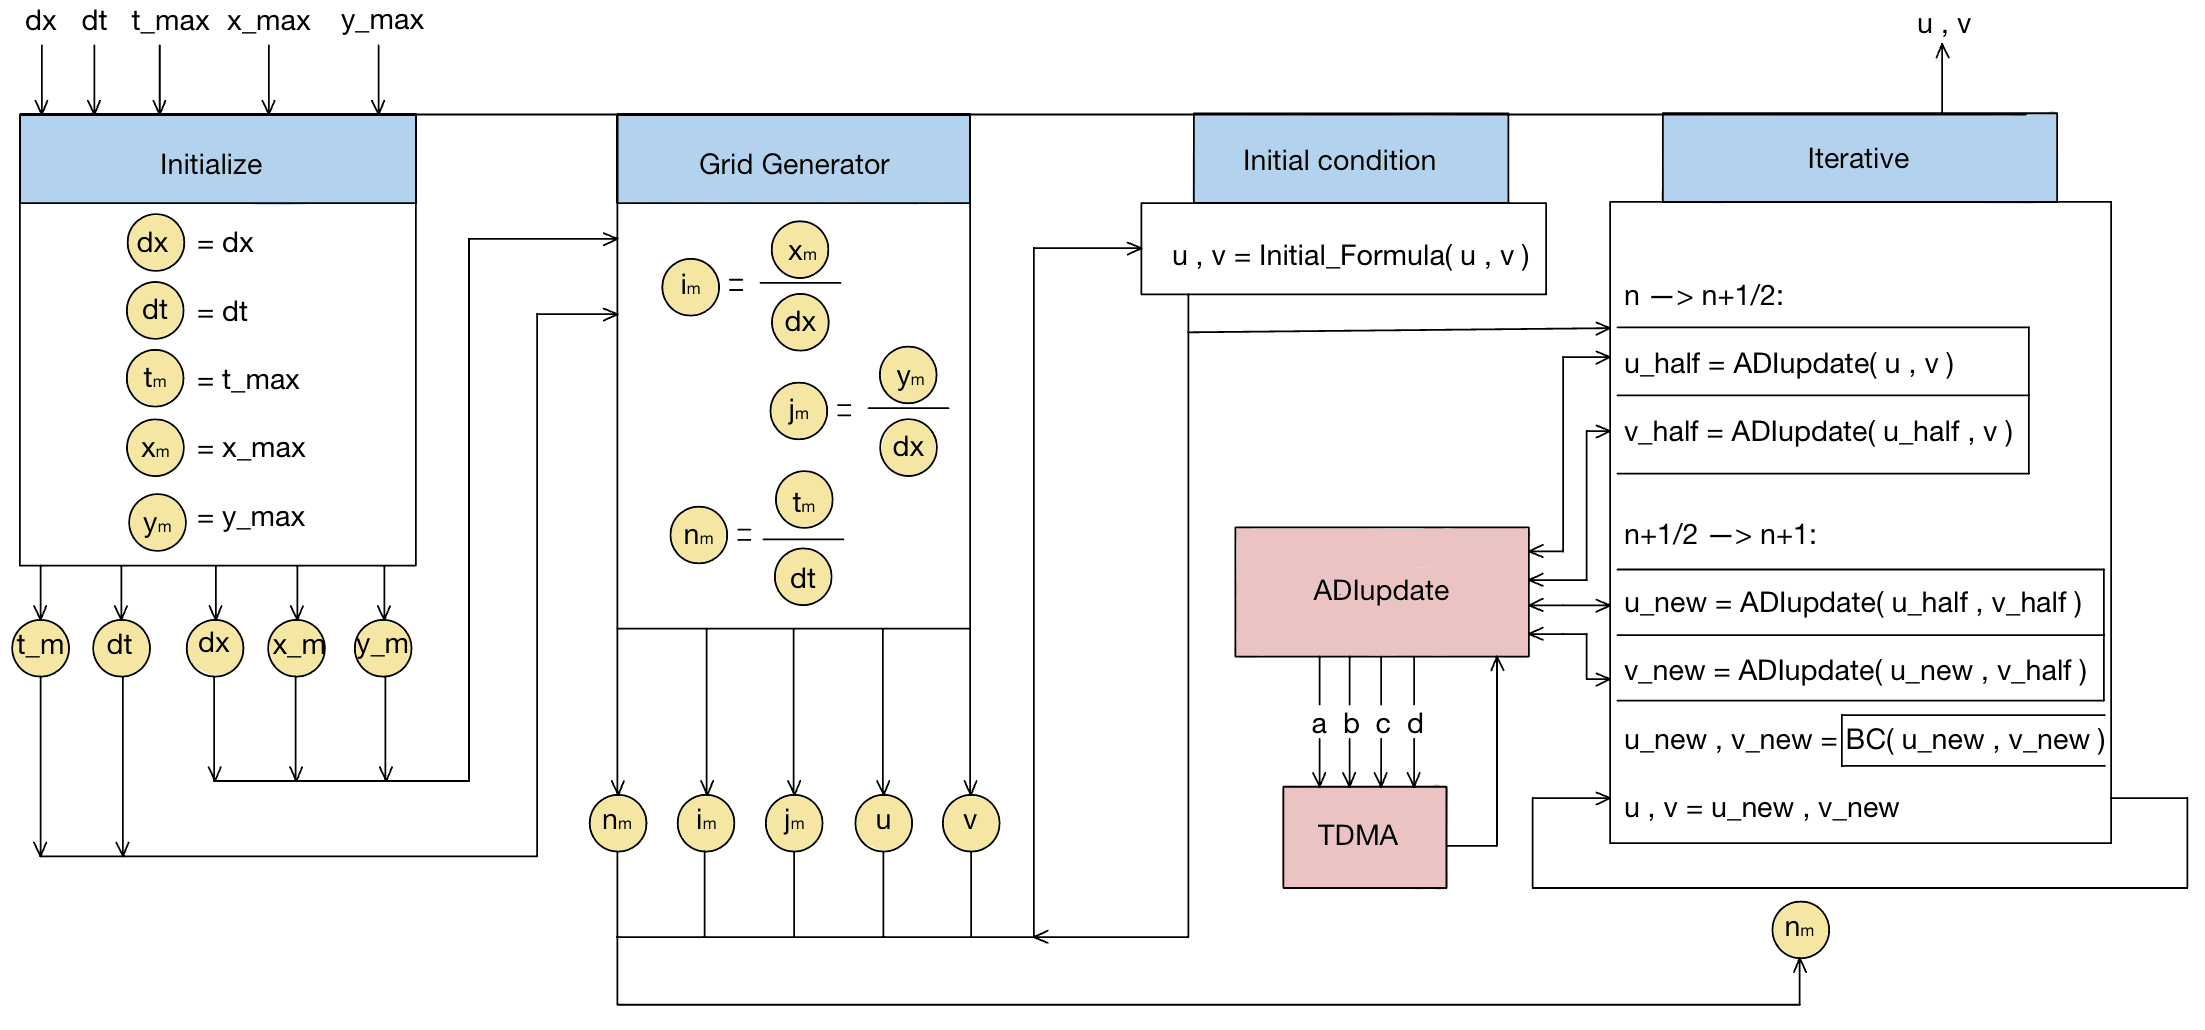
\includegraphics[width=1\textwidth]{figuresGeneral/Solver_Structure.jpg}
%     \label{IGs.jpg}
%     \caption{Solver Structure }
% \end{figure}

% % Algorithm:

% \begin{algorithm}[H]
%     \small
% \caption{xxx Method}
% \begin{algorithmic}[1]
% \For{ timestep = $n = 0$ to $N-1$} \Comment{Loop over time steps}
%     \State // Step from $n$ to $n+\frac{1}{2}$
%     \For{each each $j$ lines}  \Comment{Loop over each line}
%         \State a=b=c=($i_{max}$-1)x1 space, $a[i] = c[i] = a$, $b[i]  = b$
%         \State $U_{half}[i,j]$ = TDMA(a,b,c,d)
%     \EndFor
%     \State $U_{new}$ = BC($U_{new}$), $U = U_{new}$ 
% \EndFor

% \end{algorithmic}
% \end{algorithm}






%%%%%%%%%%%%%%%%%%%%%%%%%%%%%%%%%%%%%%%%%%%%%%%%%%%%%%%%%%%%%%%
%%%%%%%%%%%%%%%%%%%%%%%%%%%%%%%%%%%%%%%%%%%%%%%%%%%%%%%%%%%%%%%

\begin{document}

\title{\begin{Huge}Lid Driven Cavity Problem\end{Huge}\\Haobo Zhao\\530.767 CFD-HW4}
\maketitle

In this project, we developed a N-S solver for Lid Driven Cavity problem, which use $2^{nd}$ order central difference scheme in space and a second order (AB2 for convection and CN2 for viscous) fractional step in time. By separate update of the face velocity (“semi-staggered”  approach), we could approach zero divergence with the compact stencil for pressure. We also used ghost point method to obtain boundary condition. By compare our result with the reference result, we could say our result is robust.








\tableofcontents


% \section{}
% \noindent
% \begin{minipage}{0.5\linewidth}
%     \begin{flushleft}
%         u = 1, v = 0
%     \end{flushleft}
% \end{minipage}%
% \begin{minipage}{0.5\linewidth}
%     \begin{flushright}
%         u = v = 0
%     \end{flushright}
% \end{minipage}

% \vspace{5mm}

% % \begin{center}
% %     \includegraphics[width=0.5\linewidth]{cavity.png}
% % \end{center}

% \noindent
% u = v = 0
\section{Question Review}
\begin{center}
    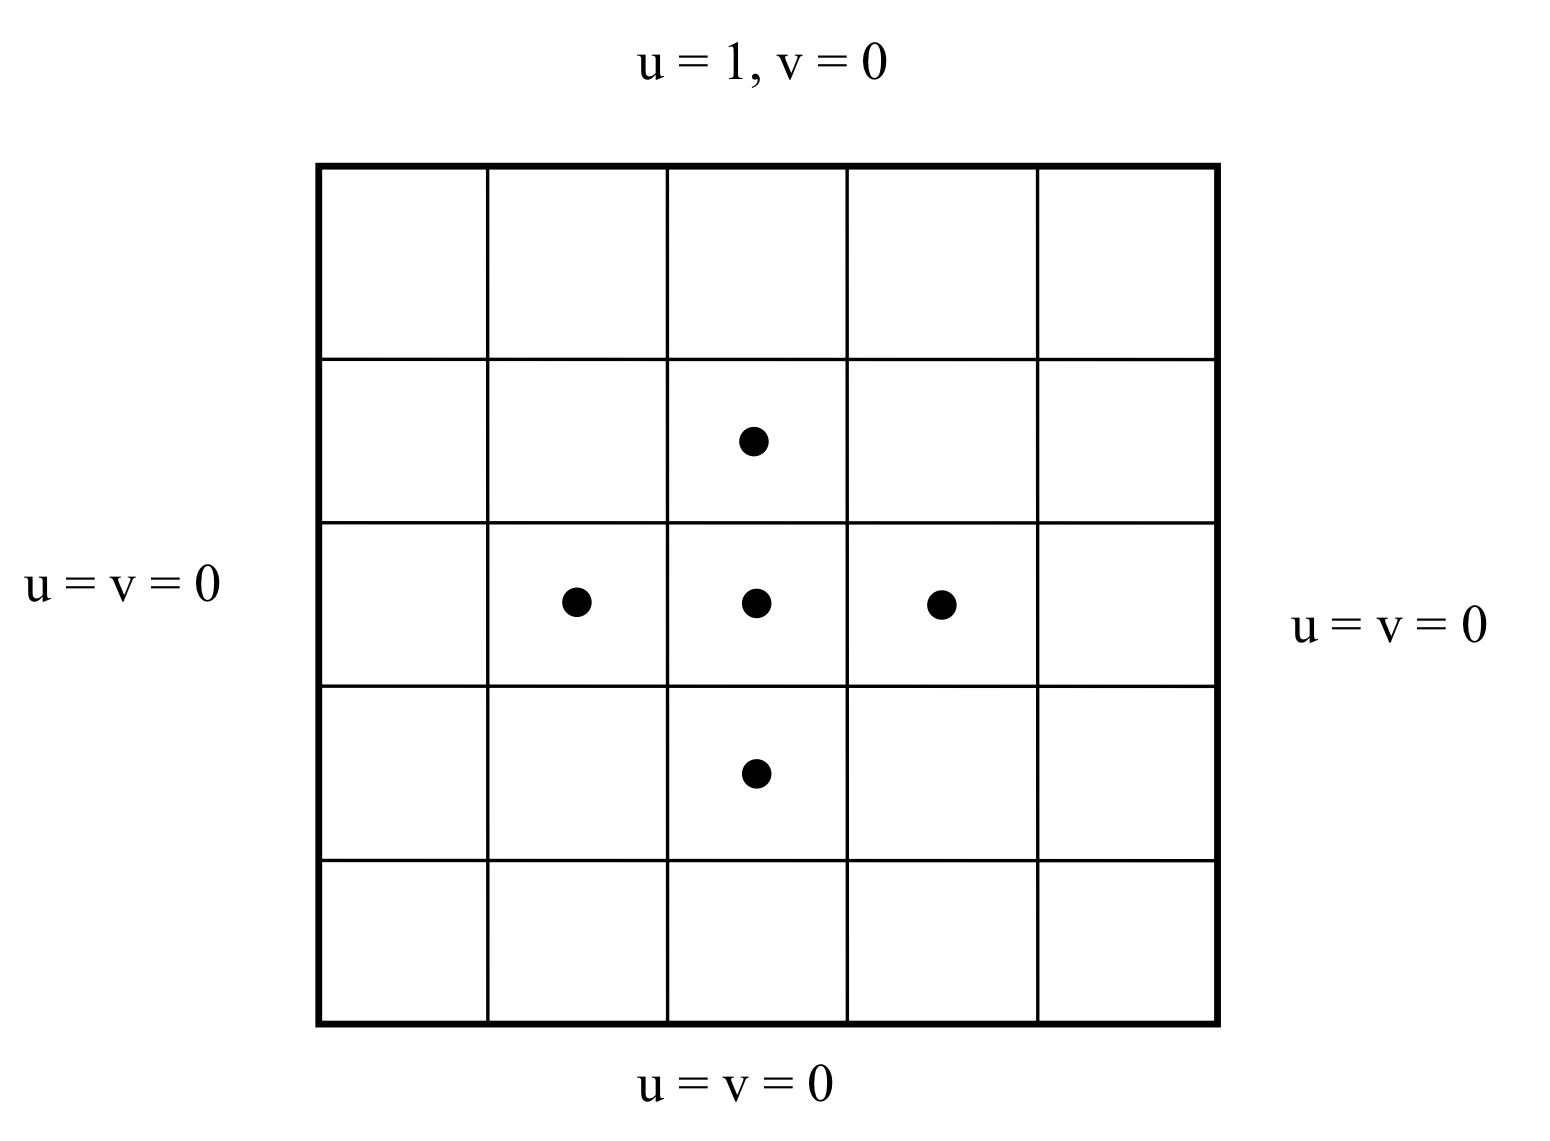
\includegraphics[width=0.6\linewidth]{figures/Question_grid.jpg}
\end{center}
Consider the \( 1 \times 1 \) cavity shown above. The cavity has a lid that moves to the right with unit velocity. This ``driven cavity'' problem is considered a benchmark in CFD and is often used to validate the fidelity and accuracy of Navier-Stokes solvers. Accurate solutions to this problem have been obtained by a number of researchers. One often quoted work in this area is that of Ghia et al. (\textit{Journal of Computational Physics}, Vol. 48, page 387, 1982)\cite{GHIA1982387}. Others include Botella, O. and Peyret, R., 1998. Benchmark spectral results on the lid-driven cavity flow. \textit{Computers \& Fluids}, 27(4), pp.421-433.\cite{BOTELLA1998421}\\




With this HW, you will start developing the code that you will also use for the Final Project

\begin{enumerate}
    \item Simulate the driven cavity flow with \( Re=100 \) on uniform grids with 16, 32, 64, 128 points in each direction. Simulate the flow until a steady state is reached. Use a 2\textsuperscript{nd} order central difference scheme in space and a second order (AB2 for convection and CN2 for viscous) fractional step in time. The basic (non-Van-Kan version of fractional step is acceptable). Use the separate update of the face velocity (``semi-staggered'' approach) so that zero divergence can be satisfied with the compact stencil for pressure.

    \item Compare your computed results (velocity profiles etc) against those from previous published studies for all grids and comment on the comparison.

    \item Compute the flow at \( Re=1000 \) and show that on a sufficiently fine mesh, your results match published results.
\end{enumerate}


% \cite{GHIA1982387}
% \cite{BOTELLA1998421}


%%%%%%%%%%%%%%%%%%%%%%%%%%%%%%%%%%%%%%%%%%%%%%%%%%%%%%
%%%%%%%%%%%%%%%%%%%%%%%%%%%%%%%%%%%%%%%%%%%%%%%%%%%%%%
%%%%%%%%%%%%%%%%%%%%%%%%%%%%%%%%%%%%%%%%%%%%%%%%%%%%%%
%%%%%%%%%%%%%%%%%%%%%%%%%%%%%%%%%%%%%%%%%%%%%%%%%%%%%%

\newpage
\section{N-S Solver}
\subsection{Discretization of N-S Equation}
The general steps solving the N-S equation is showing below:\\



\begin{tabbing}
\hspace*{2cm} \= \hspace*{2.5cm} \= \kill
\textbf{(I):} \> Using the data from the current time step and the previous time step to get $u^{*}$, $v^{*}$. \\
\> Then use $u^{*}$, $v^{*}$ to get $U^{*}$, $V^{*}$.\\


\textbf{(II):} \> Using $U^{*}$, $V^{*}$, solving the pressure poisson equation (PPE),  get $p^{n+1}$.\\


\textbf{(III):} \> Using $p^{n+1}$, and $u^{*}$, $v^{*}$, get $u^{n+1}$, $v^{n+1}$. \\
\> Using $p^{n+1}$, and $U^{*}$, $V^{*}$, get $U^{n+1}$, $V^{n+1}$.
\end{tabbing}


% (I): Using the the data we got from current time step and the pervious time step get $u^{*}$, $v^{*}$.
%     Then use $u^{*}$, $v^{*}$ get $U^{*}$, $V^{*}$.\\

% (II): using $U^{*}$, $V ^{*}$, solving pressure possion equation (PPE), get $p^{n+1}$\\

% (III): using $p^{n+1}$, and $u^{*}$, $v^{*}$, get $u^{n+1}$, $v^{n+1}$.

% using $p^{n+1}$, and $U^{*}$, $V^{*}$, get $U^{n+1}$, $V^{n+1}$.




\subsubsection{Step (I):}
Using the the data we got from current time step and the previous time step get $u^{*}$, $v^{*}$.
    Then use $u^{*}$, $v^{*}$ get $U^{*}$, $V^{*}$.\\



\textbf{Update $u^*, v^*$:}\\


The first step is going to update $u^*, v^*$:


\begin{equation}
    \frac{\vec{u}^{*} - \vec{u}^{n}}{\Delta t} = -[\frac{3}{2} \nabla \cdot (\vec{U}^n \vec{u}^{n}) - \frac{1}{2} \nabla \cdot (\vec{U}^{n-1} \vec{u}^{n-1}) ] + \frac{1}{Re} \nabla^{2} \frac{\vec{u}^*+\vec{u}^{n}}{2}
\end{equation}
    
which is:


    \begin{equation}
    \underbrace{[1 - \frac{\Delta t}{2Re}\nabla^2]\vec{u}^{*}}_{(1)} 
    = 
    -\frac{3}{2} \underbrace{[\Delta t \nabla \cdot (\vec{U}^n \vec{u}^{n})]}_{(2)} 
    + \frac{1}{2} \underbrace{[\Delta t  \nabla \cdot (\vec{U}^{n-1} \vec{u}^{n-1})]}_{(3)} 
    +\underbrace{[1+ \frac{\Delta t}{2Re} \nabla^{2}] \vec{u}}_{(4)}
\end{equation}

Could say, (2), (3) are convection term, and (4) is the diffusion term of the eqaution. 
Could use this equation to update $u^*$, $v^*$.\\


Where,
\begin{align*}
    (1) &= \left\{ 1 - \frac{\Delta t}{2Re} \nabla^2 \right\} u^{*} = P^{*} - \left[\frac{E^{*} + W^{*} - 2P^*}{\Delta x^{2}} + \frac{N^{*} + S^{*} - 2P^*}{\Delta y^{2}}\right] \frac{\Delta t}{2Re} \\
    (2) &= \frac{\Delta t}{\Delta} \left((U_{e}^{n} \frac{ E^{n} + P^{n}}{2} - U_{w}^{n} \frac{ W^{n} + P^{n}}{2}) + (V_{n}^{n} \frac{ N^{n} + P^{n}}{2} - V_{s}^{n} \frac{ S^{n} + P^{n}}{2}) \right) \\
    (3) &= \frac{\Delta t}{\Delta} \left((U_{e}^{n-1} \frac{ E^{n-1} + P^{n-1}}{2} - U_{w}^{n-1} \frac{ W^{n-1} + P^{n-1}}{2}) + (V_{n}^{n-1} \frac{ N^{n-1} + P^{n-1}}{2} - V_{s}^{n-1} \frac{ S^{n-1} + P^{n-1}}{2}) \right) \\
    (4) &= P^n + \frac{\Delta t}{2 Re \Delta^2} \left( E^{n} + W^{n} + N^{n} + S^{n} - 4P^{n} \right)
\end{align*}\\


    Could found in this expression, the formula to calculate $u^*$, $v^*$ is same, only input u or v in to the equation:\\

    $P$ means $(i,j)$, $W$ means $(i-1,j)$, $E$ means $(i+1,j)$, $S$ means $(i,j-1)$, $N$ means $(i,j+1)$.\\




\begin{figure}[H]
\centering
\begin{tikzpicture}[scale=1.5, every node/.style={scale=1}]
  % Draw grid
  \draw[step=1cm,black,thin] (1,1) grid (2,2);
  

  % Nodes for letters and coordinates
  \node at (0.5,1.5) {W};
  \node at (1.5,2.5) {N};
  \node at (1.5,1.5) {P};
  \node at (2.5,1.5) {E};
  \node at (1.5,0.5) {S};

  \node at (1,1.5) {w};
  \node at (1.5,1) {s};
  \node at (2,1.5) {e};
  \node at (1.5,2) {n};
  

  % Nodes for points
  \fill (0.5,1.5) circle[radius=0.2pt] node[below left] {$(j-1,j)$};
  \fill (1.5,2.5) circle[radius=0.2pt] node[above] {$(j,j+1)$};
  \fill (1.5,0.5) circle[radius=0.2pt] node[below] {$(j,j-1)$};
  \fill (2.5,1.5) circle[radius=0.2pt] node[below right] {$(j+1,j)$};

  % % Arrows
  % \draw[-{Latex[length=2mm]}] (1.7,1.5) -- (2.3,1.5); % Right arrow
  % \draw[-{Latex[length=2mm]}] (1.5,1.7) -- (1.5,2.3); % Up arrow
  % \draw[-{Latex[length=2mm]}] (1.3,1.5) -- (0.7,1.5); % Left arrow
  % \draw[-{Latex[length=2mm]}] (1.5,1.3) -- (1.5,0.7); % Down arrow
\end{tikzpicture}
\caption{Illustration of a grid layout with directional points.}
\end{figure}



Put the result in, could get:
$$
aW + bP + cE + eS + fN = d
$$


The left hand side is the unknown characters, and the right hand side b is known from previous and current time step. Could see, this equation in our system means $Ax = d$, where $A$ is consist of a,b,c,e,f, is a pentadiagonal matrix:


\[
\begin{bmatrix}
1 & 0 &   &   & 0 &   &    &\\
a & b & c &   &   & f &    &\\
  & a & b & c &   &   & f  &\\
  &   & a & b & c &   &    & 0\\
0 &   &   & \ddots & \ddots & \ddots &  &  \\
  & e &   &   & a & b & c &   &\\
  &   & e &   &   & a & b & c \\
  &   &   & 0 &   &   & 0 & 1 \\
\end{bmatrix}
\begin{bmatrix}
x_1 \\
x_2 \\
x_3 \\
x_4 \\
\vdots \\
x_{n-2} \\
x_{n-1} \\
x_n \\
\end{bmatrix}
=
\begin{bmatrix}
d_1 \\
d_2 \\
d_3 \\
d_4 \\
\vdots \\
d_{n-2} \\
d_{n-1} \\
d_{j\cdot i} \\
\end{bmatrix}
\]


Solve this system, we could get $u^*$, and $v^*$\\






% \[
% \begin{bmatrix}
    
%     0 & \cdots & 0 & b_{1} & c_{1} & 0 & 0 & \cdots & 0 \\
%     \vdots & & \vdots & a_{2} & b_{2} & \ddots & \ddots & \ddots & \vdots \\
%     \vdots & & \vdots & \vdots & \ddots & \ddots & c_{n-2} & 0 & \vdots \\
%     0 & \cdots & 0 & 0 & a_{n-1} & b_{n-1} & c_{n-1} & 0 & \cdots & 0 \\
%     0 & \cdots & 0 & 0 & 0 & a_{n} & b_{n} & f_{1} & 0  & 0 \\
% \end{bmatrix}
% \begin{bmatrix}
%     u_{1} \\
%     \vdots \\
%     u_{m} \\
%     u_{m+1} \\
%     \vdots \\
%     u_{m+n} \\
%     u_{m+n+1} \\
%     \vdots \\
%     u_{2m+n} \\
% \end{bmatrix}
% =
% \begin{bmatrix}
%     d_{1} \\
%     \vdots \\
%     d_{m} \\
%     d_{m+1} \\
%     \vdots \\
%     d_{m+n} \\
%     d_{m+n+1} \\
%     \vdots \\
%     d_{2m+n} \\
% \end{bmatrix}
% \]




% \[
% \begin{bmatrix}
%     e_{1} & 0 & \cdots & 0 & 0 & \cdots & 0 \\
%     0 & \ddots & \ddots & \vdots & \vdots & & \vdots \\
%     \vdots & \ddots & e_{m} & 0 & 0 & \cdots & 0 \\
%     0 & \cdots & 0 & a_{1} & b_{1} & c_{1} & 0 & \cdots & 0 \\
%     \vdots & & \vdots & a_{2} & b_{2} & \ddots & \ddots & \ddots & \vdots \\
%     \vdots & & \vdots & \vdots & \ddots & \ddots & c_{n-2} & 0 & \vdots \\
%     0 & \cdots & 0 & 0 & a_{n-1} & b_{n-1} & c_{n-1} & 0 & \cdots & 0 \\
%     0 & \cdots & 0 & 0 & 0 & a_{n} & b_{n} & f_{1} & 0 & \cdots & 0 \\
%     \vdots & & \vdots & \vdots & & \vdots & 0 & \ddots & \ddots & \ddots & \vdots \\
%     0 & \cdots & 0 & 0 & 0 & \cdots & 0 & 0 & f_{m-1} & 0 \\
%     0 & \cdots & 0 & 0 & 0 & \cdots & 0 & 0 & 0 & f_{m} \\
% \end{bmatrix}
% \begin{bmatrix}
%     u_{1} \\
%     \vdots \\
%     u_{m} \\
%     u_{m+1} \\
%     \vdots \\
%     u_{m+n} \\
%     u_{m+n+1} \\
%     \vdots \\
%     u_{2m+n} \\
% \end{bmatrix}
% =
% \begin{bmatrix}
%     d_{1} \\
%     \vdots \\
%     d_{m} \\
%     d_{m+1} \\
%     \vdots \\
%     d_{m+n} \\
%     d_{m+n+1} \\
%     \vdots \\
%     d_{2m+n} \\
% \end{bmatrix}
% \]





    % $$
    % (1) = 
    % \left\{ 1 - \frac{\Delta t}{Re} \nabla^2 \right\} u^{*} 
    % = P^{*} - [\frac{E^{*} + W^{*}-2P^*}{\Delta x^{2}} + \frac{N^{*} + S^{*}-2P^*}{\Delta y^{2}}] \frac{\Delta t}{Re}
    % $$ 

    % $$
    % (2) = 
    % \frac{\Delta t}{\Delta } \left((U_{e}^{n} \frac{ E^{n} + P^{n}}{2} - U_{w}^{n} \frac{ W^{n} + P^{n}}{2})  
    % + (V_{n}^{n} \frac{ N^{n} + P^{n}}{2} - V_{s}^{n} \frac{ S^{n} + P^{n}}{2}) \right)
    % $$
    
    % $$
    % (3) = 
    % \frac{\Delta t}{\Delta } \left((U_{e}^{n-1} \frac{ E^{n-1} + P^{n-1}}{2} - U_{w}^{n-1} \frac{ W^{n-1} + P^{n-1}}{2})  
    % + (V_{n}^{n-1} \frac{ N^{n-1} + P^{n-1}}{2} - V_{s}^{n-1} \frac{ S^{n-1} + P^{n-1}}{2}) \right)
    % $$
    
    % $$
    % (4) = P^n + \frac{\Delta t}{2 Re \Delta^2} \left( E^{n} + W^{n} + N^{n} + S^{n} - 4P^{n} \right)
    % $$

    




\textbf{Update $U^*, V^*$:}\\
    $$ U_e^* = \frac{u_p^*+u_E^*}{2} , V_n^* = \frac{v_P^*+v_N^*}{2}$$


\subsubsection{Step (II):}
\textbf{Update $p^{n+1}$:}\\

$$
    \nabla^2 p = \frac{\nabla \cdot \vec{u}^*}{\Delta t}= \frac{\frac{U_e^* - U_P^*}{\Delta x} + \frac{V_n^* - V_s^*}{\Delta y}}{\Delta t}
$$

$$
\frac{P_E + P_W - 2P_P}{\Delta x^2} + \frac{P_N + P_S - 2P_P}{\Delta y^2} = \frac{\frac{U_e^* - U_w^*}{\Delta x} + \frac{V_n^* - V_s^*}{\Delta y}}{\Delta t}
$$

$$
P_E + P_W + P_N + P_S - 4P_P = \frac{\Delta}{\Delta t} \left( U_e^* - U_w^* + V_n^* - V_s^* \right) = RHS
$$

Similarly, this equation also give us a pentadiagonal system:


\[
\begin{bmatrix}
1 & 0 &   &   & 0 &   &    &\\
a & b & c &   &   & f &    &\\
  & a & b & c &   &   & f  &\\
  &   & a & b & c &   &    & 0\\
0 &   &   & \ddots & \ddots & \ddots &  &  \\
  & e &   &   & a & b & c &   &\\
  &   & e &   &   & a & b & c \\
  &   &   & 0 &   &   & 0 & 1 \\
\end{bmatrix}
\begin{bmatrix}
x_1 \\
x_2 \\
x_3 \\
x_4 \\
\vdots \\
x_{n-2} \\
x_{n-1} \\
x_n \\
\end{bmatrix}
=
\begin{bmatrix}
d_1 \\
d_2 \\
d_3 \\
d_4 \\
\vdots \\
d_{n-2} \\
d_{n-1} \\
d_n \\
\end{bmatrix}
\]



% $$
% \begin{bmatrix}
%     1 & D &   &   &  \\
%     D & \ddots & D &   &  \\
%       & D & \ddots & D &  \\
%       &   & D & 1 & D \\
%       &   &   & D & 1 \\
%     \end{bmatrix}
%     \begin{bmatrix}
%     \phi_1 \\
%     \phi_2 \\
%     \vdots \\
%     \phi_{n-1} \\
%     \phi_n \\
%     \end{bmatrix}
%     =
%     \begin{bmatrix}
%     b_1 \\
%     b_2 \\
%     \vdots \\
%     b_{n-1} \\
%     b_n \\
%     \end{bmatrix}
% $$



\subsubsection{Step (III):}
\textbf{Update $u^{n+1}$, $v^{n+1}$:}\\
The equation to update the $u^{n+1}$, $v^{n+1}$ is showing below:
$$
\vec{u}^{n+1} = \vec{u}^* - \Delta t (\nabla p)_{cc}
$$
where we could calculate the cell center pressure divergence $(\nabla p)_{cc}$, and:

$$
\begin{cases}
    u^{n+1} = u^* - \Delta t \cdot \frac{P_E - P_W}{2\Delta x} \\
    v^{n+1} = v^* - \Delta t \cdot \frac{P_N - P_S}{2\Delta y}
\end{cases}
$$


\textbf{Update $U^{n+1}$, $V^{n+1}$:}\\
The equation to update the $U^{n+1}$, $V^{n+1}$ is showing below:
$$
\vec{U}^{n+1} = \vec{U}^* - \Delta t (\nabla p)_{fc}
$$

where we could calculate the face center pressure divergence $(\nabla p)_{fc}$, and:


$$
\begin{cases}
    U_{e}^{n+1} = U_{e}^* - \Delta t \cdot \frac{P_E - P_P}{\Delta x} \\
    V_{n}^{n+1} = V_{n}^* - \Delta t \cdot \frac{P_N - P_P}{\Delta y}
    \end{cases}
$$

\subsubsection{LineSOR implementation}
In the discretization steps (I) and (II) of the Navier-Stokes equations, we obtain a pentadiagonal matrix system. However, our Tridiagonal Matrix Algorithm (TDMA) can only solve systems represented by tridiagonal matrices. To address this, we transfer the additional diagonal lines, e and f, to the right-hand side and continue iterating. This process is repeated until the results satisfy the original requirements of the pentadiagonal system.



\textbf{The origional pentadiagonal system:}\\

\[
\begin{bmatrix}
1 & 0 &   &   & 0 &   &    &\\
a & b & c &   &   & f &    &\\
  & a & b & c &   &   & f  &\\
  &   & a & b & c &   &    & 0\\
0 &   &   & \ddots & \ddots & \ddots &  &  \\
  & e &   &   & a & b & c &   &\\
  &   & e &   &   & a & b & c \\
  &   &   & 0 &   &   & 0 & 1 \\
\end{bmatrix}
\begin{bmatrix}
u_1 \\
u_2 \\
u_3 \\
u_4 \\
\vdots \\
u_{n-2} \\
u_{n-1} \\
u_n \\
\end{bmatrix}
=
\begin{bmatrix}
d_1 \\
d_2 \\
d_3 \\
d_4 \\
\vdots \\
d_{n-2} \\
d_{n-1} \\
d_n \\
\end{bmatrix}
\]


% \[
% \begin{bmatrix}
% 1 & 0 &   &   &  &   &    &\\
% a & b & c &   &   &  &    &\\
%   & a & b & c &   &   &   &\\
%   &   & a & b & c &   &    & \\
%  &   &   & \ddots & \ddots & \ddots &  &  \\
%   &  &   &   & a & b & c &   &\\
%   &   &  &   &   & a & b & c \\
%   &   &   &  &   &   & 0 & 1 \\
% \end{bmatrix}
% \begin{bmatrix}
% u_1 \\
% u_2 \\
% u_3 \\
% u_4 \\
% \vdots \\
% u_{n-2} \\
% u_{n-1} \\
% u_n \\
% \end{bmatrix}
% =
% \begin{bmatrix}
% d_1 \\
% d_2 \\
% d_3 \\
% d_4 \\
% \vdots \\
% d_{n-2} \\
% d_{n-1} \\
% d_n \\
% \end{bmatrix}
% \]

























For each line j, the system could be represented as:

\[
\left[
\begin{array}{c|c|c}
E & T & F 
\end{array}
\right]
\begin{bmatrix}
    [u_{j-1}^{n+1}] \\
    [u_{j}^{n+1}] \\
   [ u_{j+1}^{n+1}]
\end{bmatrix}
=
\begin{bmatrix}
    [d_{j}] \\
\end{bmatrix}
\]

Could say, E mans operating the previous line (j-1) to current line (j), and F means operating on the next line (j+1) to current line. Where $\left[
\begin{array}{c|c|c}
E & T & F 
\end{array}
\right]$ is:


\[
\left[
\begin{array}{cccccc|cccccc|cccccc}
0 & 0 & \cdots & 0 & 0 & 0 & 1 & 0 & 0 & \cdots & 0 & 0 & 0 & 0 & \cdots & 0 & 0 & 0 \\
0 & e_{2} & 0 & \cdots & 0 & 0 & a_{2} & b_{2} & c_{2} & \ddots & \vdots & 0 & 0 & f_{2} & 0 & \cdots & 0 & 0 \\
0 & 0 & e_{3} & \cdots & 0 & 0 & 0 & a_{3} & \ddots & \ddots & 0 & 0 & 0 & 0 & f_{3} & \cdots & 0 & 0 \\
0 & \vdots & \vdots & \ddots & \vdots & \vdots & \vdots & \ddots & \ddots & \ddots & c_{2} & 0 & 0 & \vdots & \vdots & \ddots & \vdots & \vdots \\
0 & 0 & 0 & \cdots & e_{n-1} & 0 & 0 & \ddots & \ddots & 0 & b_{n-1} & c_{n-1} & 0 & 0 & 0 & \cdots & f_{n-1} & 0 \\
0 & 0 & 0 & \cdots & 0 & 0 & 0 & \cdots & 0 & 0 & 0 & 1 & 0 & 0 & 0 & \cdots & 0 & 0 \\
\end{array}
\right]
\]\\

\textbf{LineSOR:}\\

For LineSOR, we move the two diagonal line (e and f) to the right hand side:

\[
\left[
\begin{array}{c|c|c}
0 & T & 0 
\end{array}
\right]
\begin{bmatrix}
    [u_{j-1}^{k+1}] \\
    [u_{j}^{k+1}] \\
   [ u_{j+1}^{k+1}]
\end{bmatrix}
=
\begin{bmatrix}
    [d_{j}] \\
\end{bmatrix}
-
\left[
\begin{array}{c|c|c}
E & 0 & F 
\end{array}
\right]
\begin{bmatrix}
    [u_{j-1}^{k}] \\
    [u_{j}^{k}] \\
   [ u_{j+1}^{k}]
\end{bmatrix}
\]


Which is:

\[
\left[
T
\right]
\begin{bmatrix}
    [u_{j}^{k+1}]
\end{bmatrix}
=
\begin{bmatrix}
    [d_{j}] \\
\end{bmatrix}
-
\left[
E
\right]
\begin{bmatrix}
    [u_{j-1}^{k}]
\end{bmatrix}
-
\left[
F
\right]
\begin{bmatrix}
    [u_{j+1}^{k}]
\end{bmatrix}
\]







Where we could use TDMA to solve this equation. As this result is different from directly solve the equation we previously got, we need it keep iterating, until the error small enough:


\[ 
Error = 
\left[
\begin{array}{c|c|c}
E & T & F 
\end{array}
\right]
\begin{bmatrix}
    [u_{j-1}^{k+1}] \\
    [u_{j}^{k+1}] \\
   [ u_{j+1}^{k+1}]
\end{bmatrix}
-
\begin{bmatrix}
    [d_{j}] \\
\end{bmatrix}
<1e-6
\]


%%%%%%%%%%%%%%%%%%%%%%%%%%%%%%%%%%%%%%%%%%%%%%%%%%%%%%

\subsection{Setting}
\subsubsection{Solver field}
As in the discretization of N-S equation, we have $u$, $v$, $p$, and $U$, $V$ fields. To handle boundary condition, we use ghost point. For convenient, we set all the fields in same size: $(N+2) \cdot (N+2)$, the u, v, p fields are:

\begin{figure}[H]
    \centering
    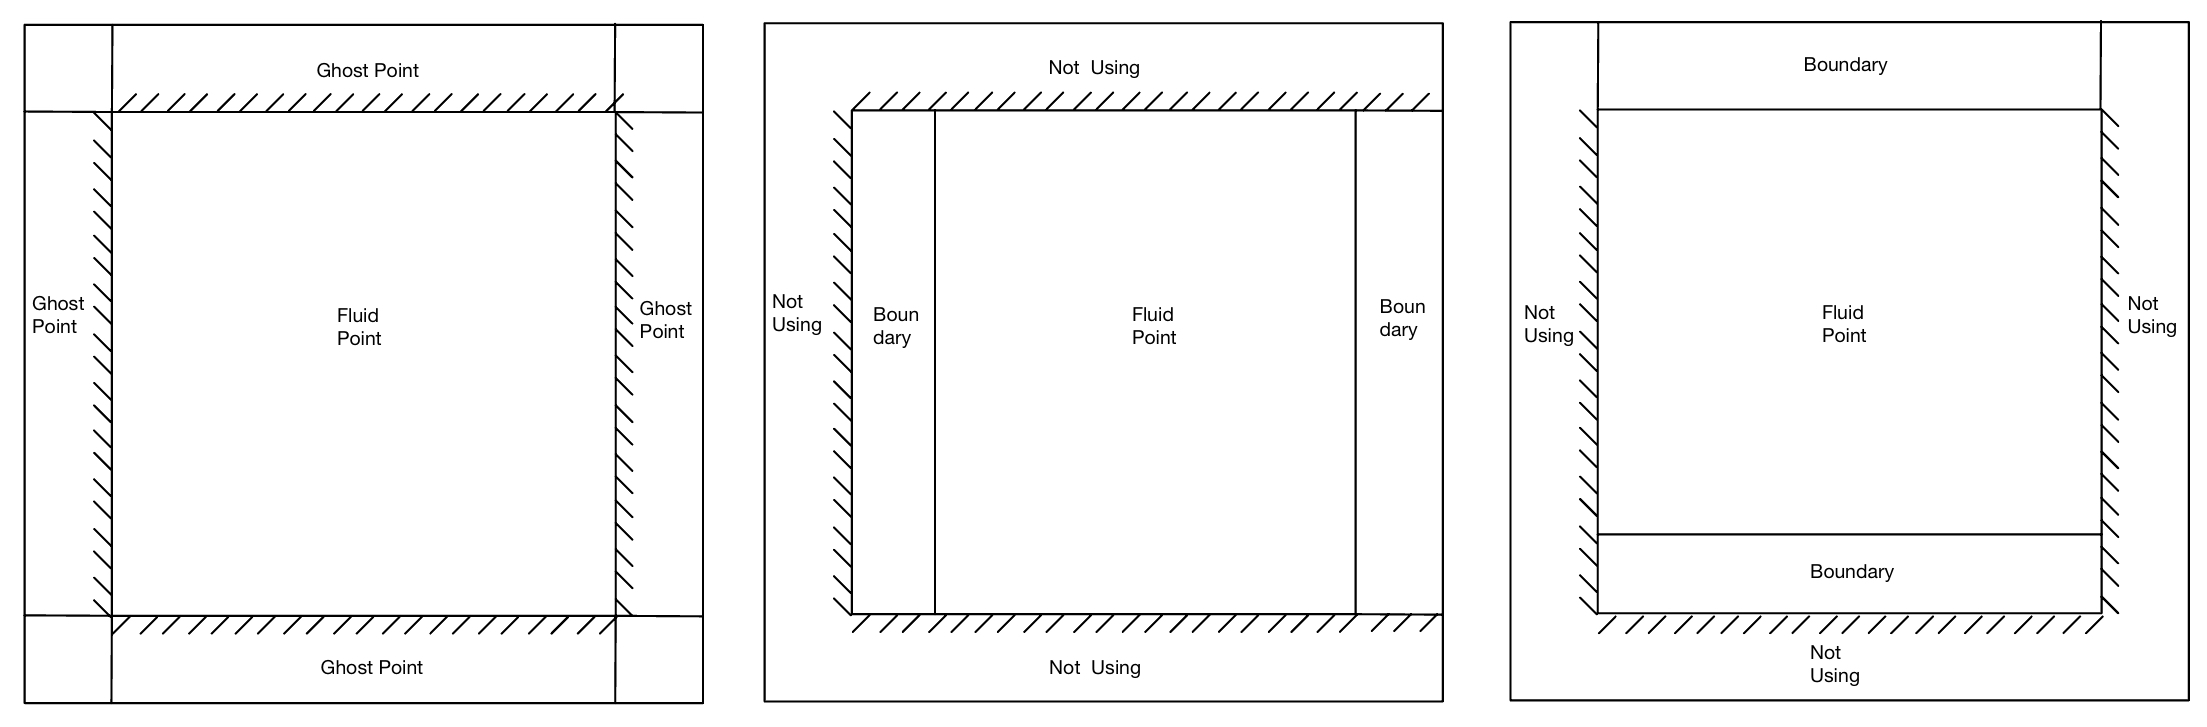
\includegraphics[width=0.9\linewidth]{Homeworks/HW4-Lid_Driven_Cavity/Latex/figures/Solver/Domain.jpg}
    \caption{u/v/p, U, and V field}
\end{figure}

The left one is for u, v, and p field, where they are defined at cell center. It contains ghost point, which is in the solid part near to the boundary. U field is in the middle, which is 1 column, and 2 rows less than u/v/p field. V field is the right one, where it is 1 row, and 2 column less than u/v/p field.


\begin{figure}[H]
\centering
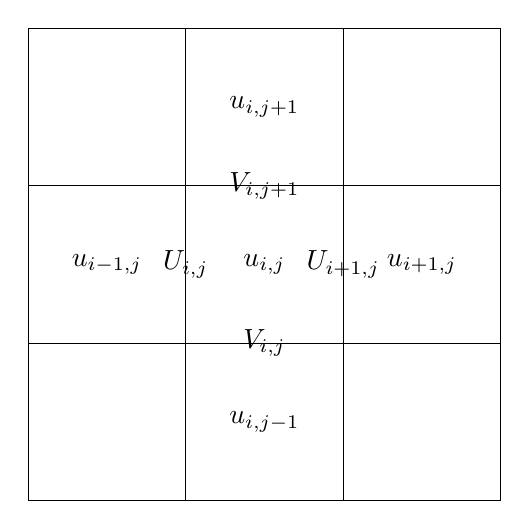
\begin{tikzpicture}[scale=2, every node/.style={scale=1}]
  % Draw grid
  \draw[step=1cm,black,thin] (0,0) grid (3,3);
  

  % Nodes for letters and coordinates
  \node at (0.5,1.5) {$u_{i-1,j}$};
  \node at (1.5,2.5) {$u_{i,j+1}$};
  \node at (1.5,1.5) {$u_{i,j}$};
  \node at (2.5,1.5) {$u_{i+1,j}$};
  \node at (1.5,0.5) {$u_{i,j-1}$};

  \node at (1,1.5) {$U_{i,j}$};
  \node at (1.5,1) {$V_{i,j}$};
  \node at (2,1.5) {$U_{i+1,j}$};
  \node at (1.5,2) {$V_{i,j+1}$};
  
\end{tikzpicture}
\caption{Illustration of a grid layout with u/v/p, U, and V.}
\end{figure}


\subsubsection{Boundary condition and implementation}
First, let us clarify boundary condition:
Both 4 sides are in dirichlet boundary condition.
Which means at the boundary point:

$$
\frac{u_{p} + u_{gs}}{2} = u_{B}
$$















\subsection{Solver Architecture}
\begin{figure}[H]
    \centering
    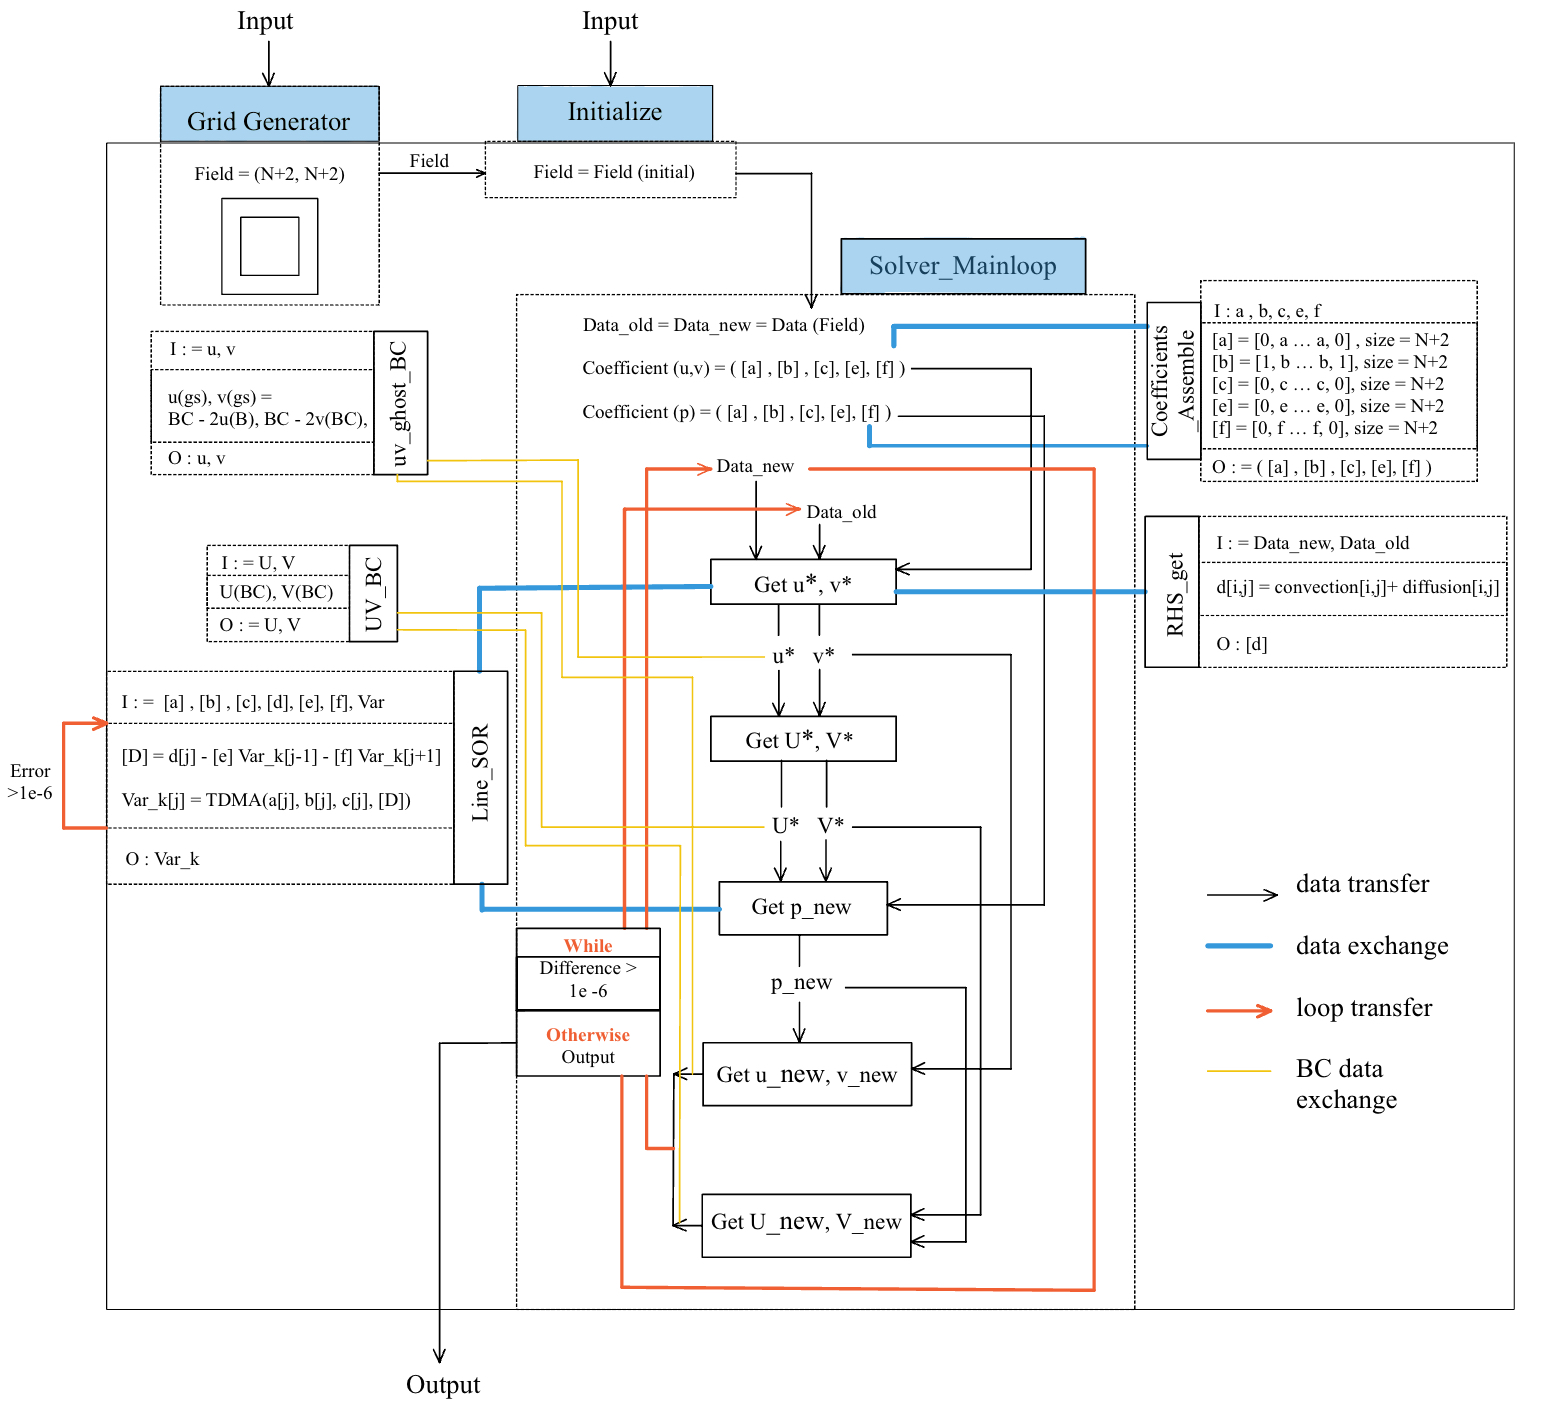
\includegraphics[width=1\linewidth]{Homeworks/HW4-Lid_Driven_Cavity/Latex/figures/Solver/Solver_Architecture.jpg}
    \caption{Solver Architecture}
\end{figure}


This diagram shows our Solver structure. By Using grid generator to generate fields for $u, v, p$, and $U, V$, transfer the data to initialize the initial value, then use the main loop to doing time iteration till the fields get to steady state, we could output the result. \\

\begin{itemize}
    \item \textbf{I/O}: I means function input, and O means function output.
    \item \textbf{Data Transfer Lines}: The diagram uses different colored lines to indicate various types of data movement, while the lines with arrow means one-way data transfer, which means value assignment, and the lines without arrow means data exchange, where there is data input to function, but there is also data get back from function.
\end{itemize}

















\newpage
\section{Result for Re=100}
\subsection{Stream lines at Re=100}
For Re=100, we got the result after the flow reaches steady state, where we use the total difference of u, v, and p smaller than 1e-6, we could get the streamlines results in different grid size showing below:
\begin{figure}[H]
    \centering
    \begin{subfigure}[b]{0.48\linewidth}
        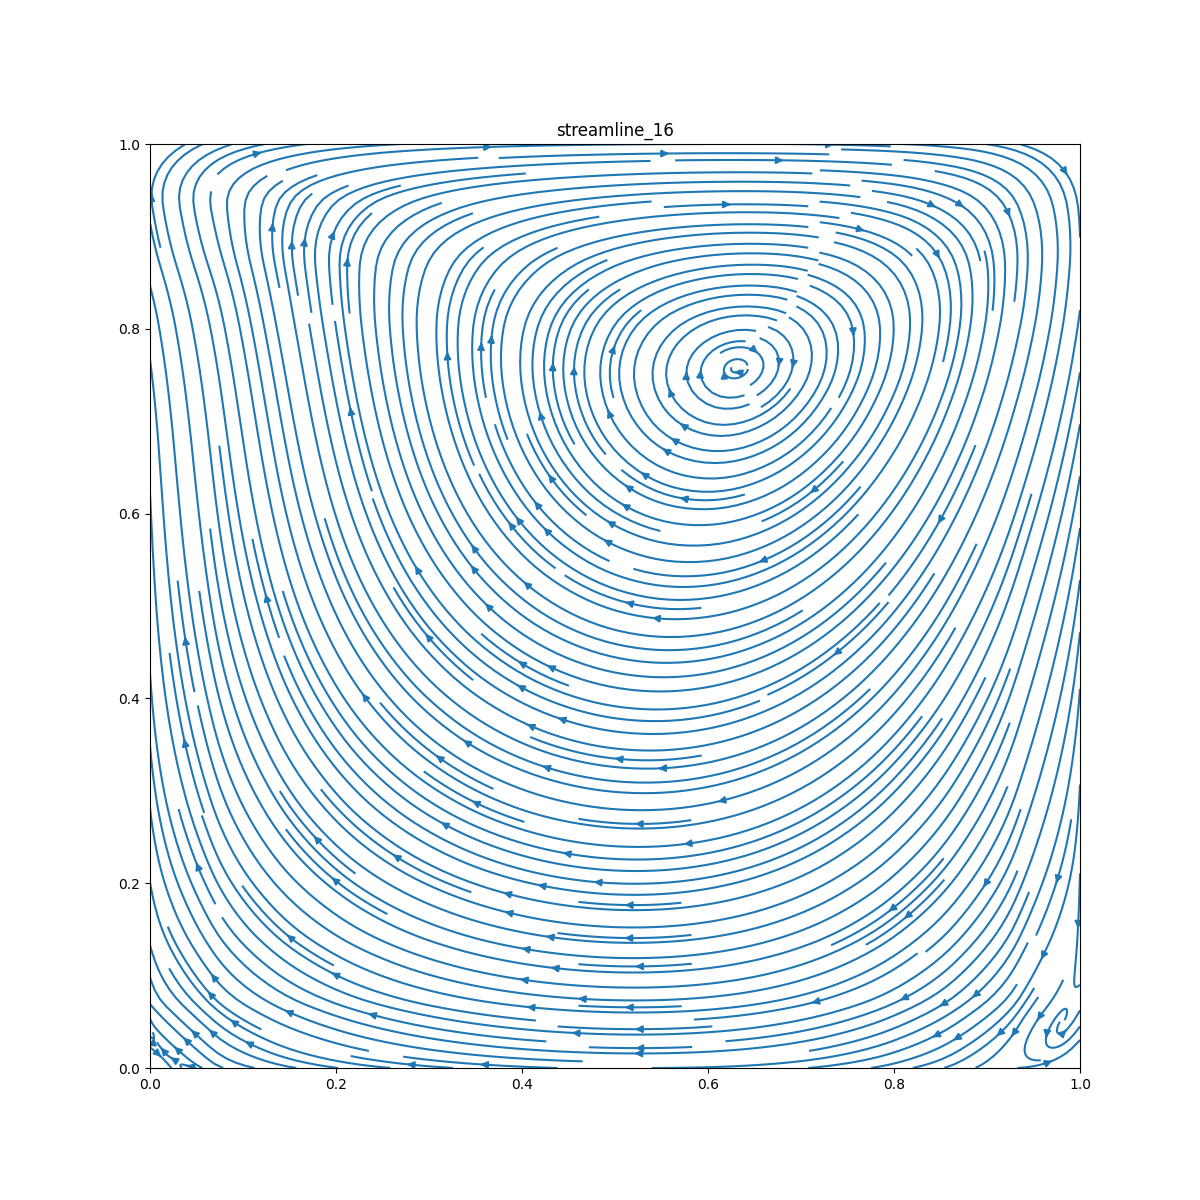
\includegraphics[width=\linewidth]{figures/Re=100_result/streamline_16.png}
        \caption{N=16}
    \end{subfigure}
    \hspace{-5mm} % Reduce horizontal space
    \begin{subfigure}[b]{0.48\linewidth}
        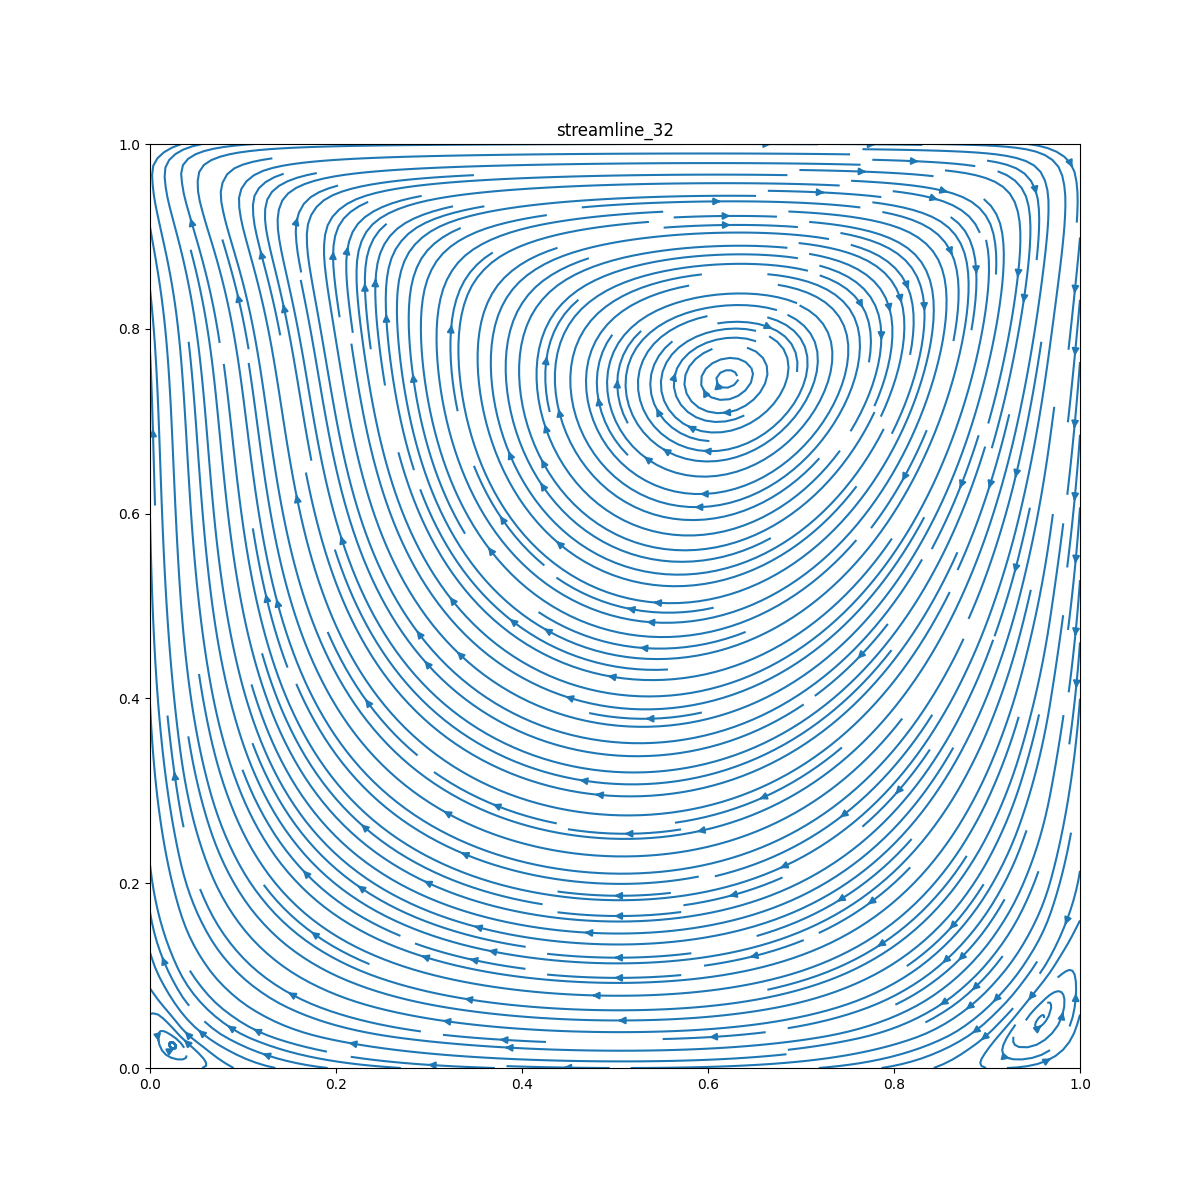
\includegraphics[width=\linewidth]{figures/Re=100_result/streamline_32.png}
        \caption{N=32}
    \end{subfigure}
    
    \begin{subfigure}[b]{0.48\linewidth}
        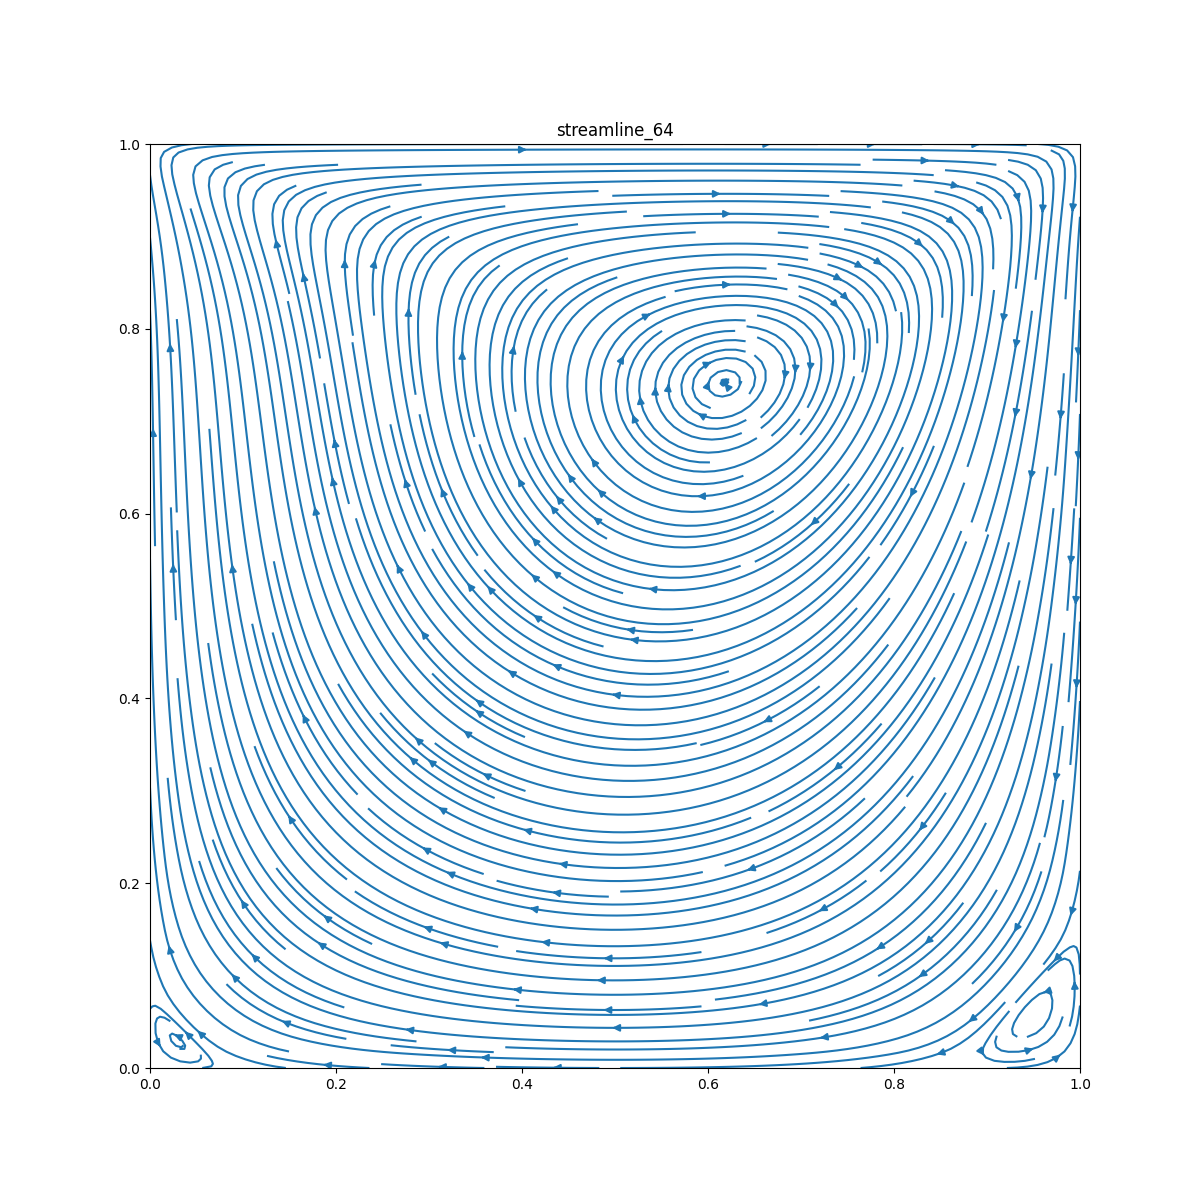
\includegraphics[width=\linewidth]{figures/Re=100_result/streamline_64.png}
        \caption{N=64}
    \end{subfigure}
    \hspace{-5mm} % Reduce horizontal space
    \begin{subfigure}[b]{0.48\linewidth}
        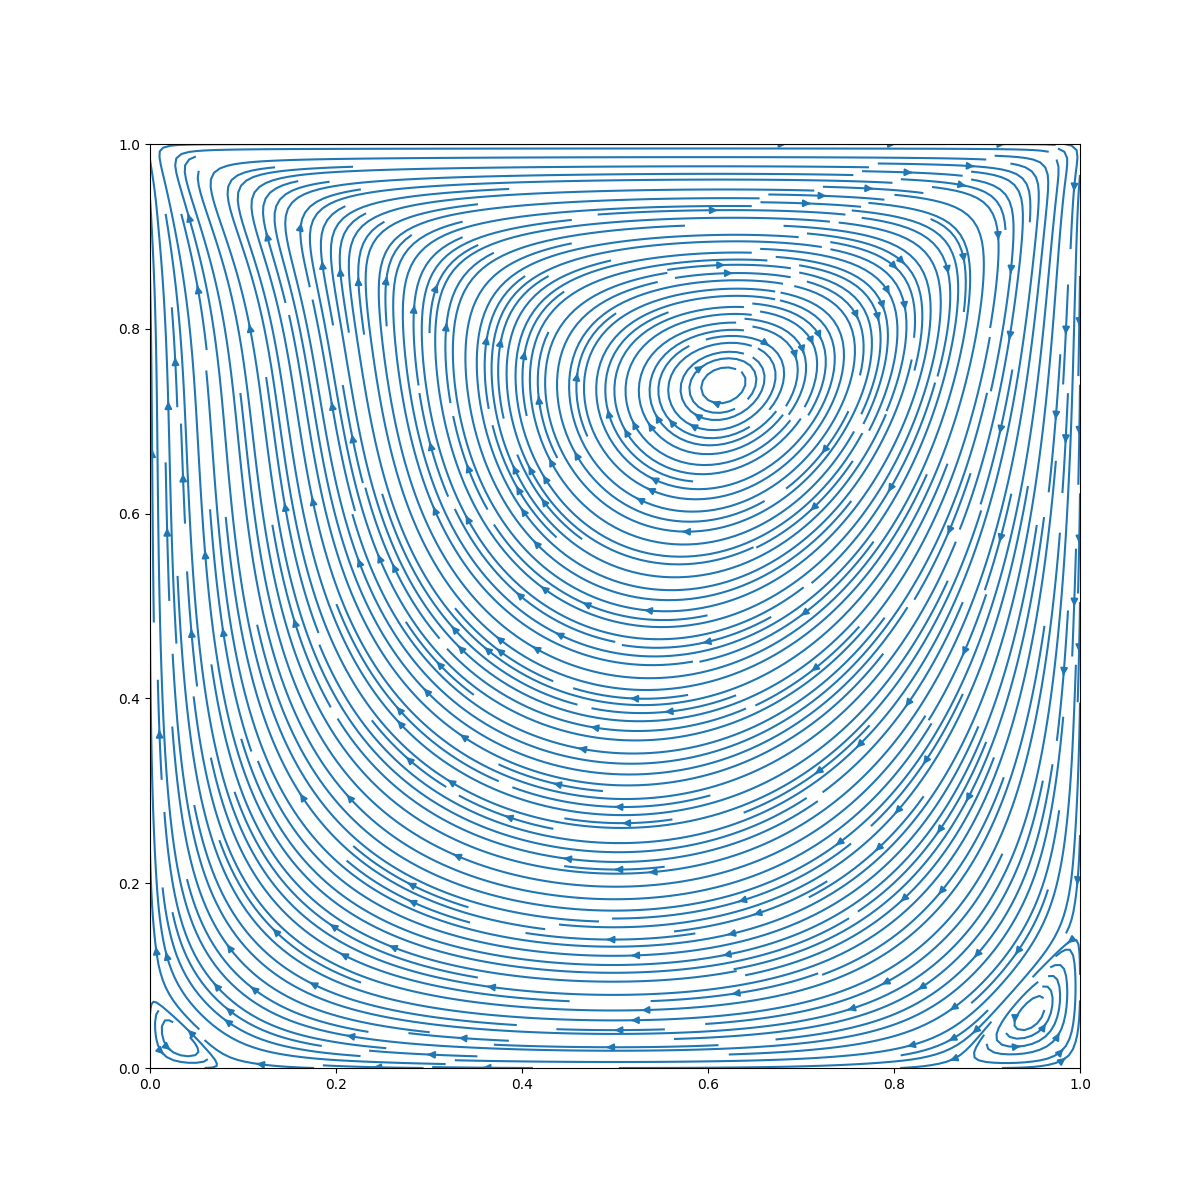
\includegraphics[width=\linewidth]{figures/Re=100_result/streamline_128.png}
        \caption{N=128}
    \end{subfigure}
    \caption{Stream line visualizations at different grid resolutions}
\end{figure}

For general view, we could see there is a big vortex appear at the biased center of the cavity, 
and the small vortex represent at 
the left bottom and a relatively larger vortex appear at the  right bottom of the cavity.\\


\subsubsection{Streamline comparison of different grid size result}
Compare different grid size result, 
we could find that for N=16 grid, 
the vortex at left bottom is not showing,
 and the vortex on the right bottom is small. 
 Where as the grid become finer, 
 the vortex shows up and the vortex at 
 the right bottom become larger.







\subsection{Result comparison to the reference}

To make our result is robust, we compare the result with the reference (Ghia et al, 1982)\cite{GHIA1982387}. The results is showing below:

\subsubsection{Streamline comparison}
\begin{figure}[H]
    \centering
    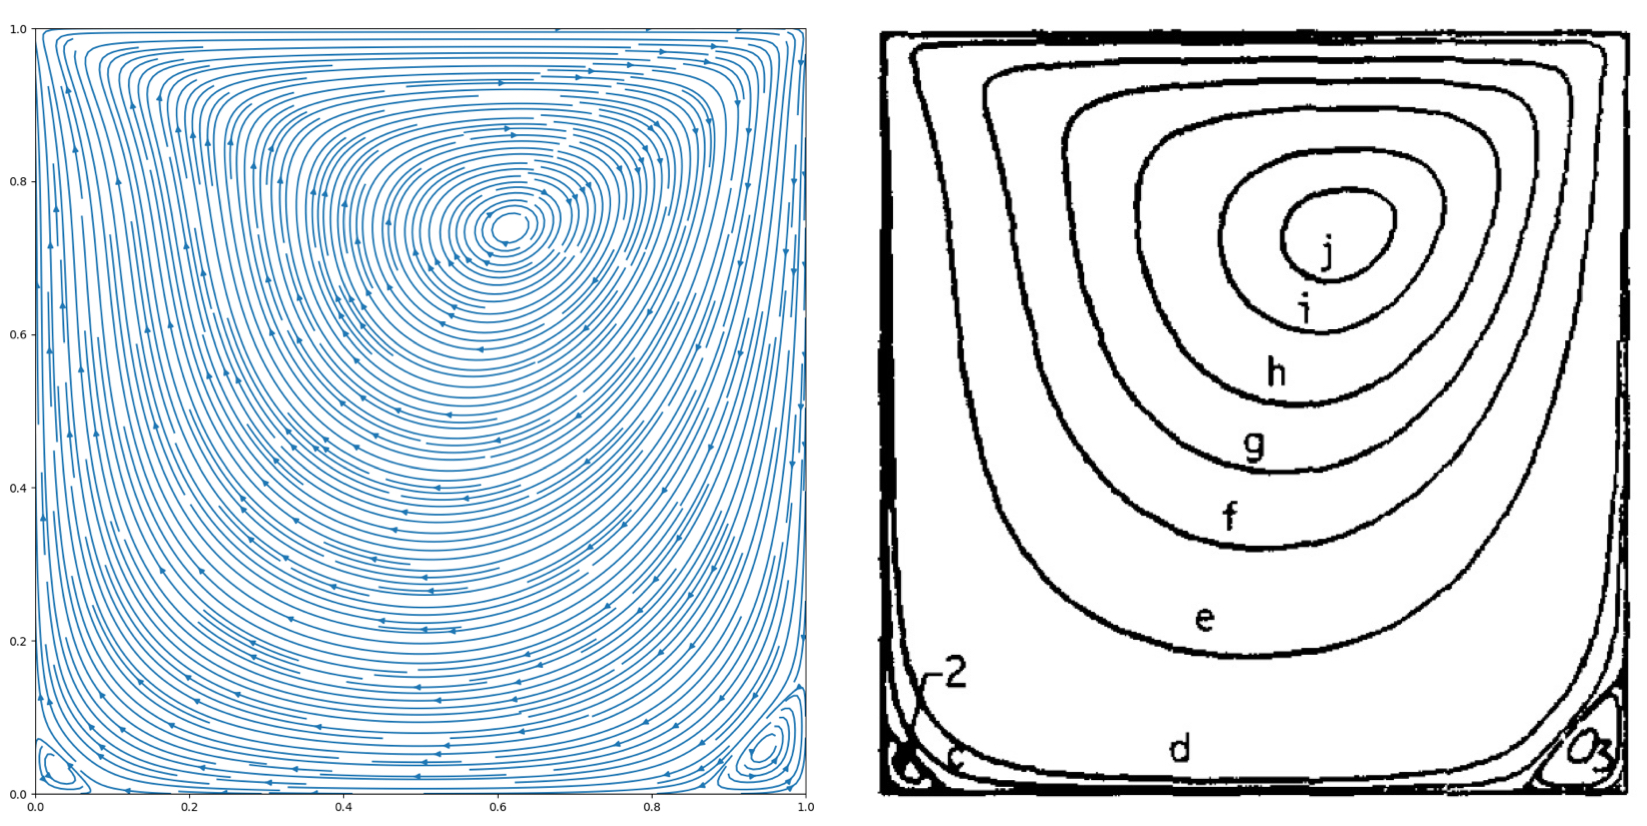
\includegraphics[width=0.9\linewidth]{Homeworks/HW4-Lid_Driven_Cavity/Latex/figures/Re=100_result/Compare.jpg}
    \caption{left: Result Streamline, right: Ghia(1982)\cite{GHIA1982387}'s result}
\end{figure}

Compare out N=128 result to the Ghia (1982)\cite{GHIA1982387} 's result, we could find the results is similar, where the there shows three vortex, and the stream lines are similar.

\subsubsection{Velocity at geometry center}


Measure our result's accuracy need us to compare the result with the reference (Ghia et al. 1982)\cite{GHIA1982387}. By compare the result at geometry center, we could check the accuracy of our result. 







\begin{figure}[H]
    \centering
    \begin{tikzpicture}
        \node[anchor=south west,inner sep=0] (image) at (0,0) {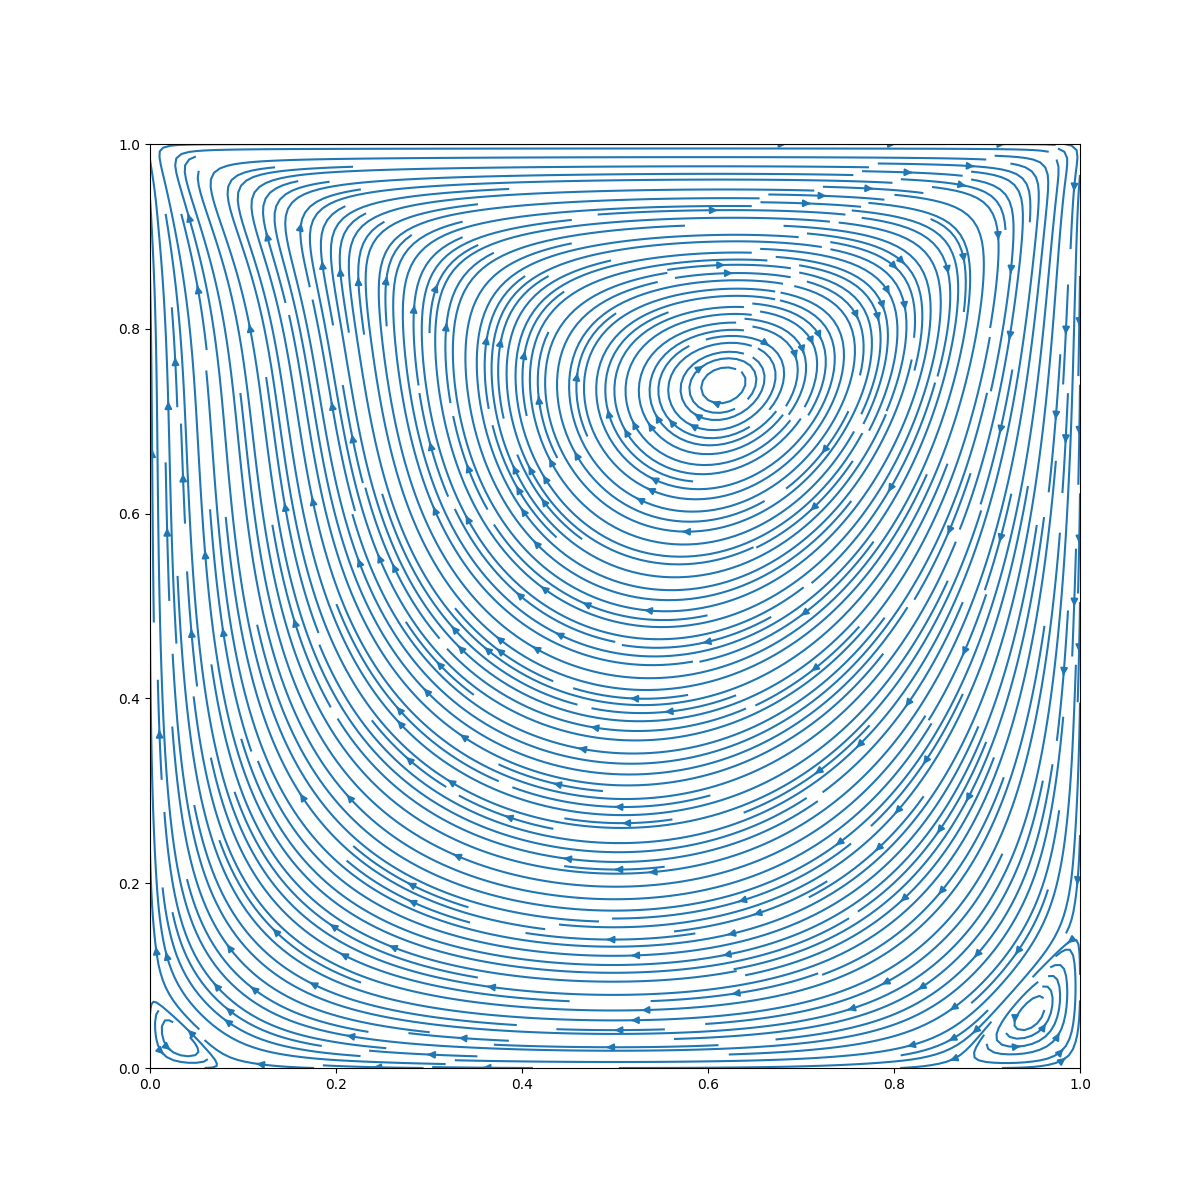
\includegraphics[width=0.6\textwidth]{figures/Re=100_result/streamline_128.png}};
        \begin{scope}[x={(image.south east)},y={(image.north west)}]
            % horizontal line
            \draw[black, thick] (0.1,0.5) -- (0.9,0.5);
            \node[anchor=south, align= center, text width=2cm] at (1,0.5) {v at vertical center};
            % vertical line
            \draw[black, thick] (0.5,0.1) -- (0.5,0.9);
            \node[anchor=south] at (0.5,0.05) {u at horizontal center};
        \end{scope}
    \end{tikzpicture}
    \caption{velocity at geometry center}
\end{figure}


We use the the horizontal velocity u at horizontal center (at same vertical line, middle at horizontal), and vertical velocity v at vertical center (at same horizontal line, middle at horizontal). The general result is showing below:


\begin{figure}[H]
    \centering
    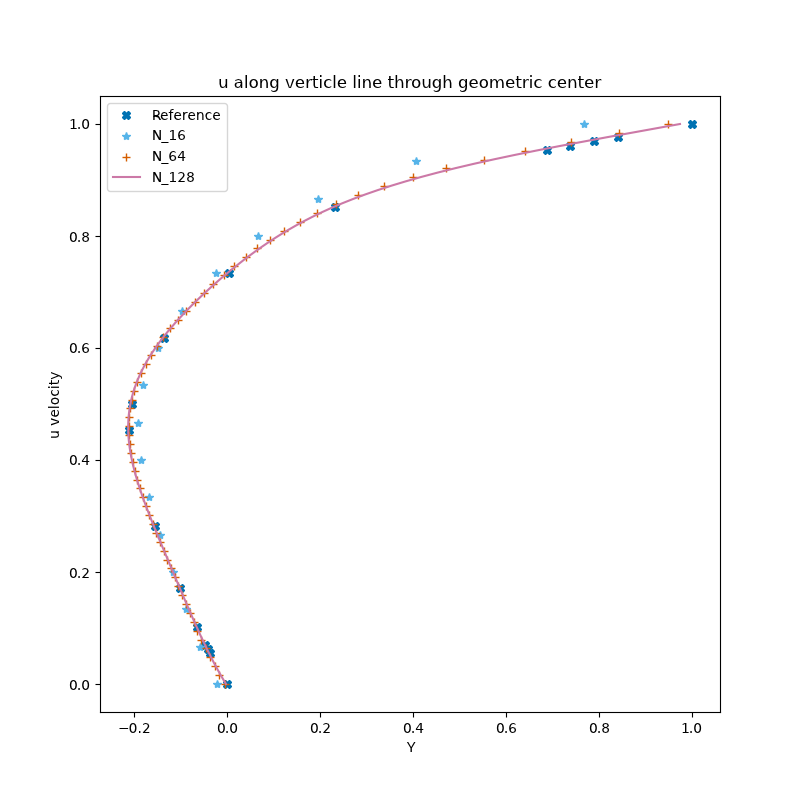
\includegraphics[width=0.5\linewidth]{figures/u along verticle line through geometric center.png}
    \hspace{-8mm} % Reduce horizontal space
    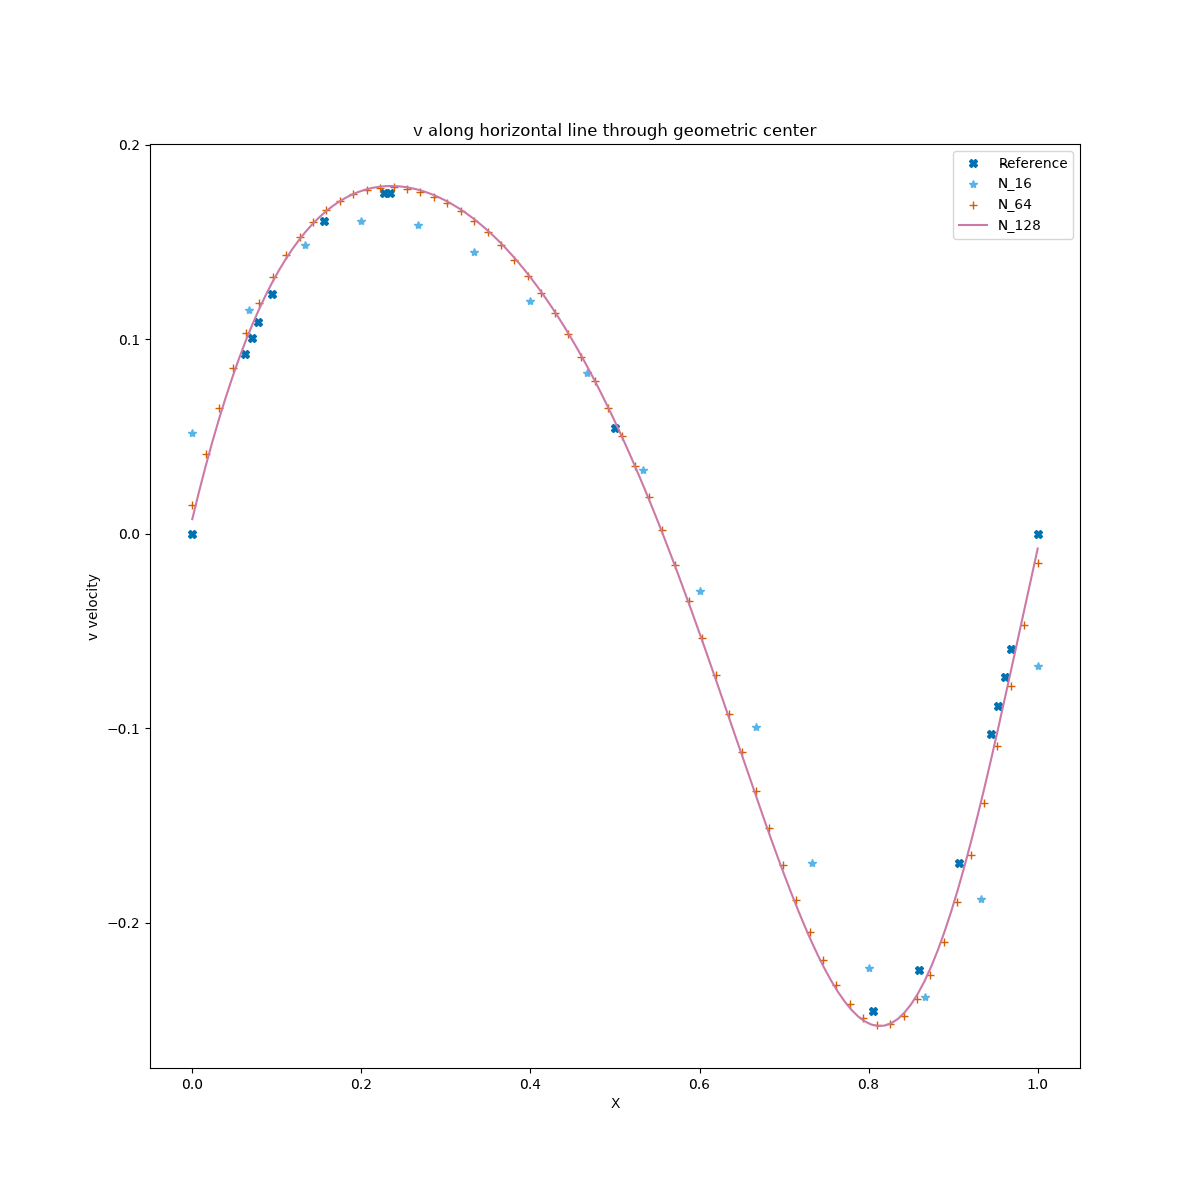
\includegraphics[width=0.5\linewidth]{figures/v along horizontal line through geometric center.png }
    \caption{u along vertical line at middle of x (left), v along horizontal line at middle of y (right). Reference is Ghia (1982)\cite{GHIA1982387}'s result. There is also enlarged figures showing down below.}
\end{figure}


\begin{figure}[H]
    \centering
    \begin{tikzpicture}[spy using outlines={circle, magnification=2, size=6cm, connect spies}]
        \node {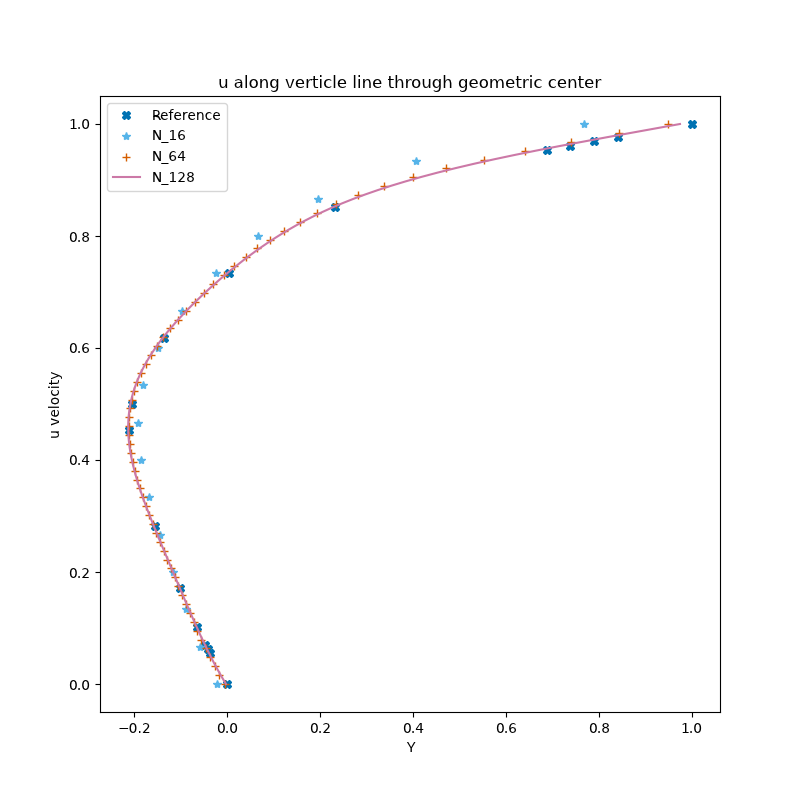
\includegraphics[width=0.6\textwidth]{figures/u along verticle line through geometric center.png}};
        \spy on (-2.2cm, 0cm) in node [left] at (6cm, -1cm);
    \end{tikzpicture}
    \caption{u along vertical line at middle of x (large)}
\end{figure}

This figures shows velocity u at the horizontal middle of the domain. Could say, in general the result is matching. Also compare different grid size, could find the coarsest grid, N=16, biased largest from reference result. Conversely, the finest grid, N=128, match pretty good.


\begin{figure}[H]
    \centering
    \begin{tikzpicture}[spy using outlines={circle, magnification=2, size=4cm, connect spies}]
        \node {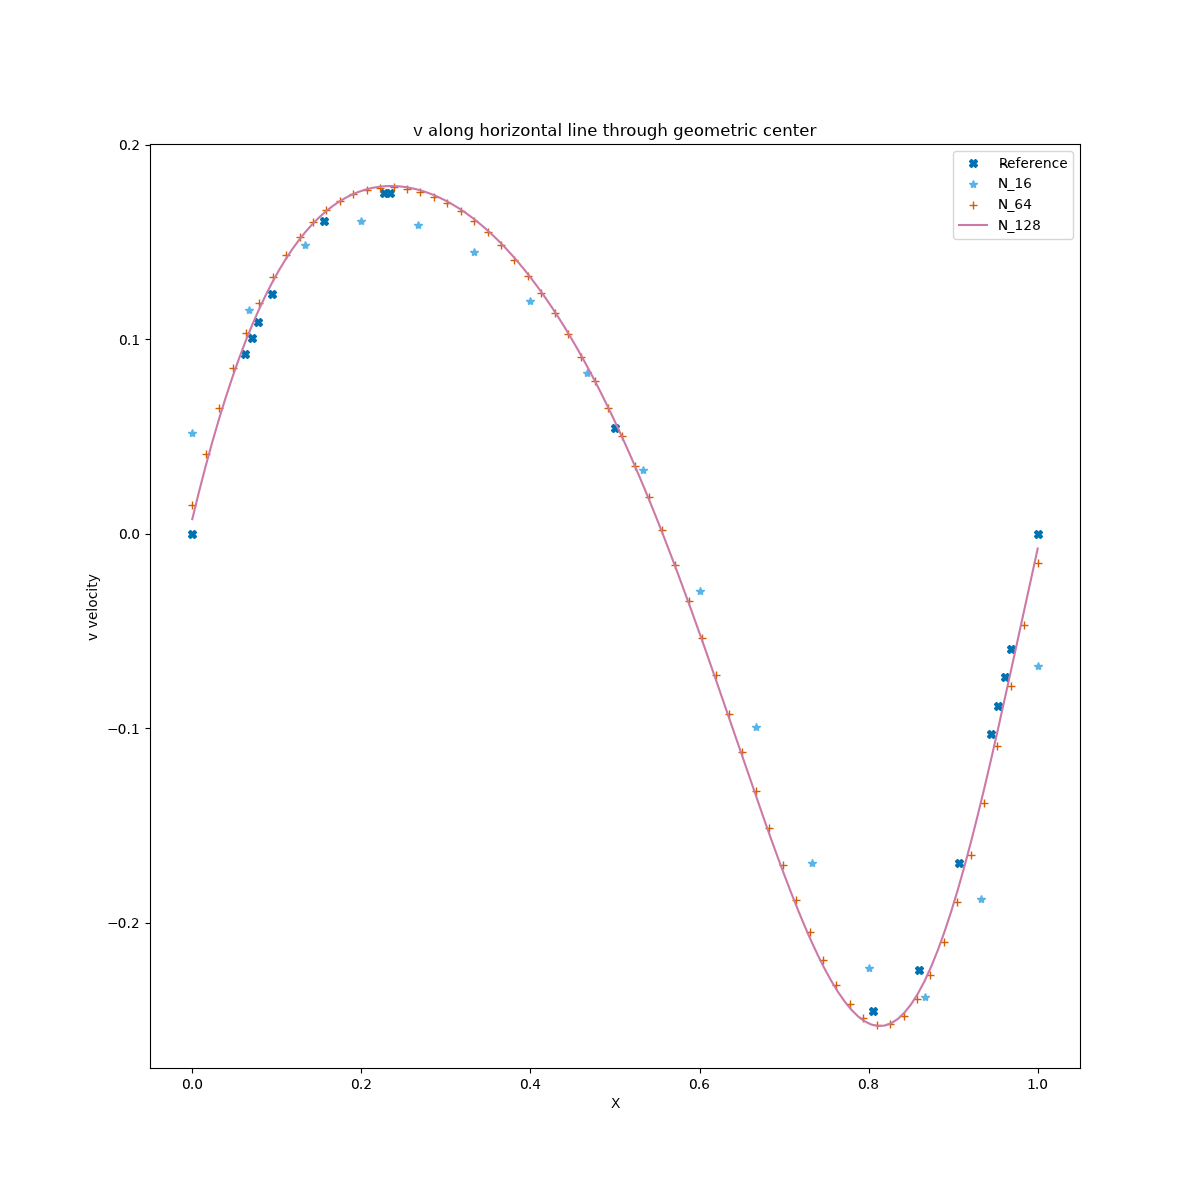
\includegraphics[width=0.6\textwidth]{figures/v along horizontal line through geometric center.png}};
        \spy on (-1.8cm, 2.6cm) in node [left] at (0cm, -1.5cm);
        \spy on (2.6cm, -2.7cm) in node [right] at (3.5cm, 2cm);
    \end{tikzpicture}
    \caption{v along horizontal line at middle of y (large)}
\end{figure}


Could find in these solution, that the N = 16 grid is the most rough grid, where the difference with the paper result (N=128) is the largest.
The finest grid (N=128) us the most accurate grid, where the result match the result from paper.  

As the grid become finer, the result become more accurate.























\section{Result for Re=1000}
\subsection{Stream lines at Re=1000}
For Re=1000, the streamlines result is showing below:
\begin{figure}[H]
    \centering
    \begin{subfigure}[b]{0.48\linewidth}
        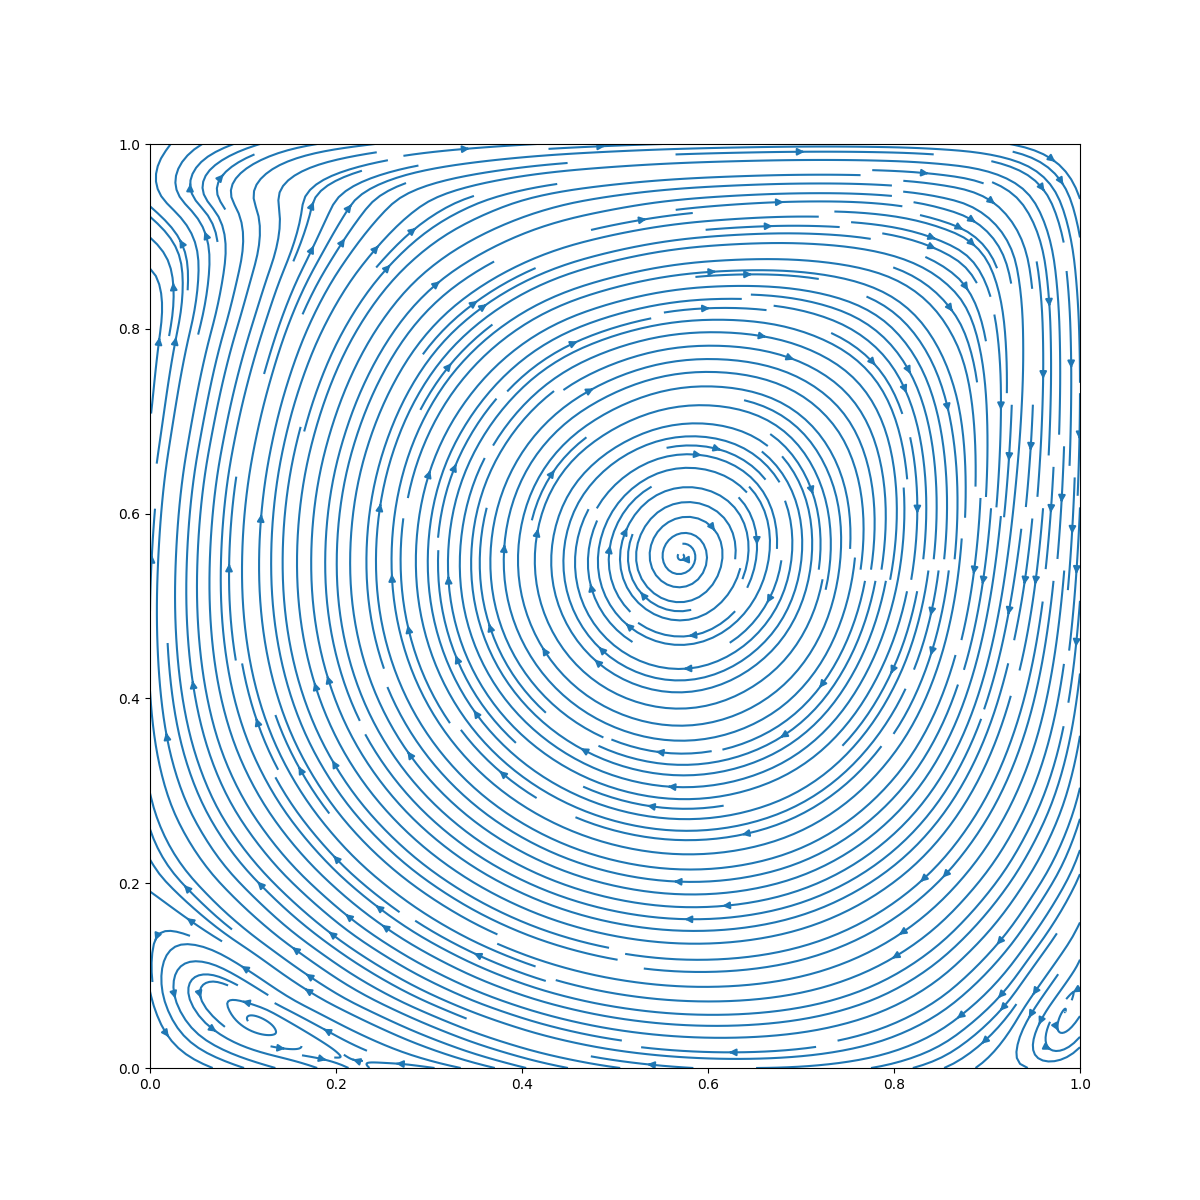
\includegraphics[width=\linewidth]{figures/Re=1000_result/Re1000_streamline_16.png}
        \caption{N=16}
    \end{subfigure}
    \hspace{-5mm} % Reduce horizontal space
    \begin{subfigure}[b]{0.48\linewidth}
        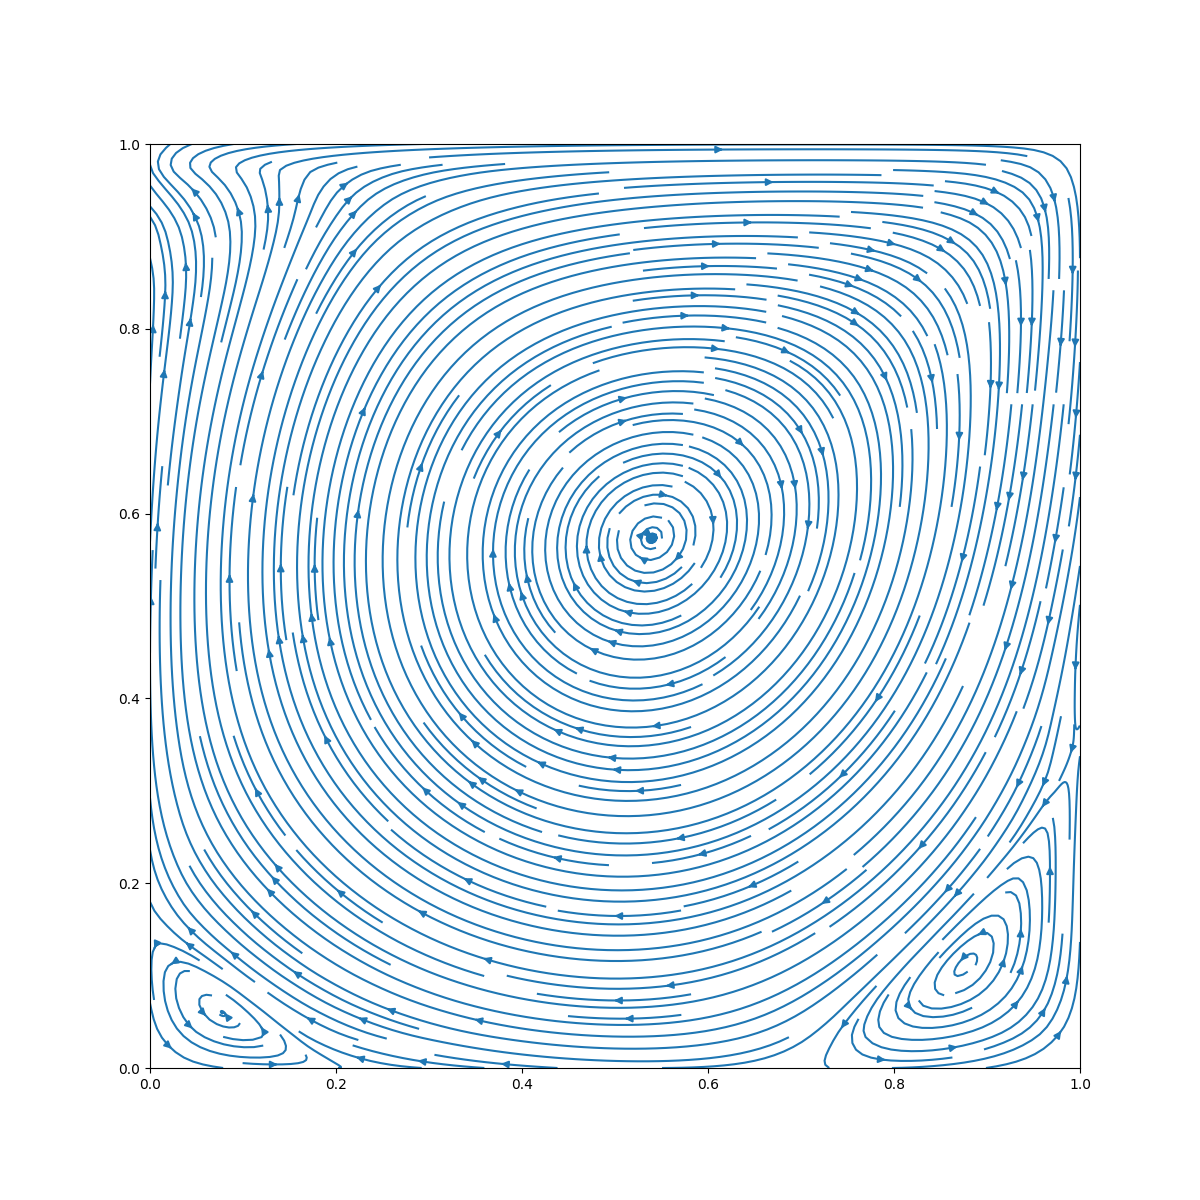
\includegraphics[width=\linewidth]{figures/Re=1000_result/Re1000_streamline_32.png}
        \caption{N=32}
    \end{subfigure}
    
    \begin{subfigure}[b]{0.48\linewidth}
        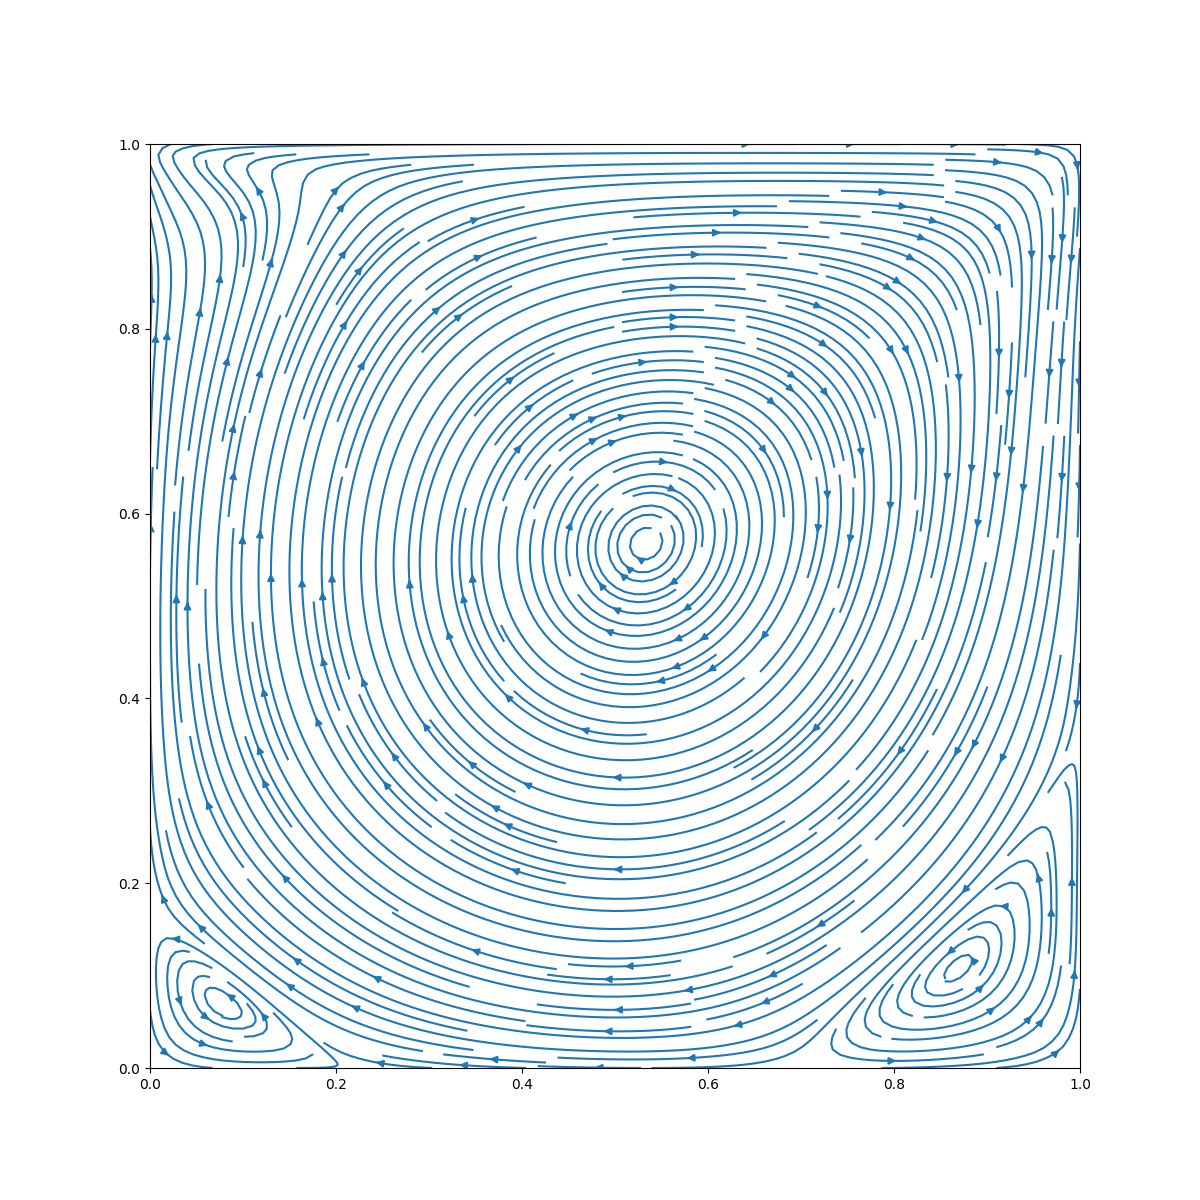
\includegraphics[width=\linewidth]{figures/Re=1000_result/Re1000_streamline_64.png}
        \caption{N=64}
    \end{subfigure}
    \hspace{-5mm} % Reduce horizontal space
    \begin{subfigure}[b]{0.48\linewidth}
        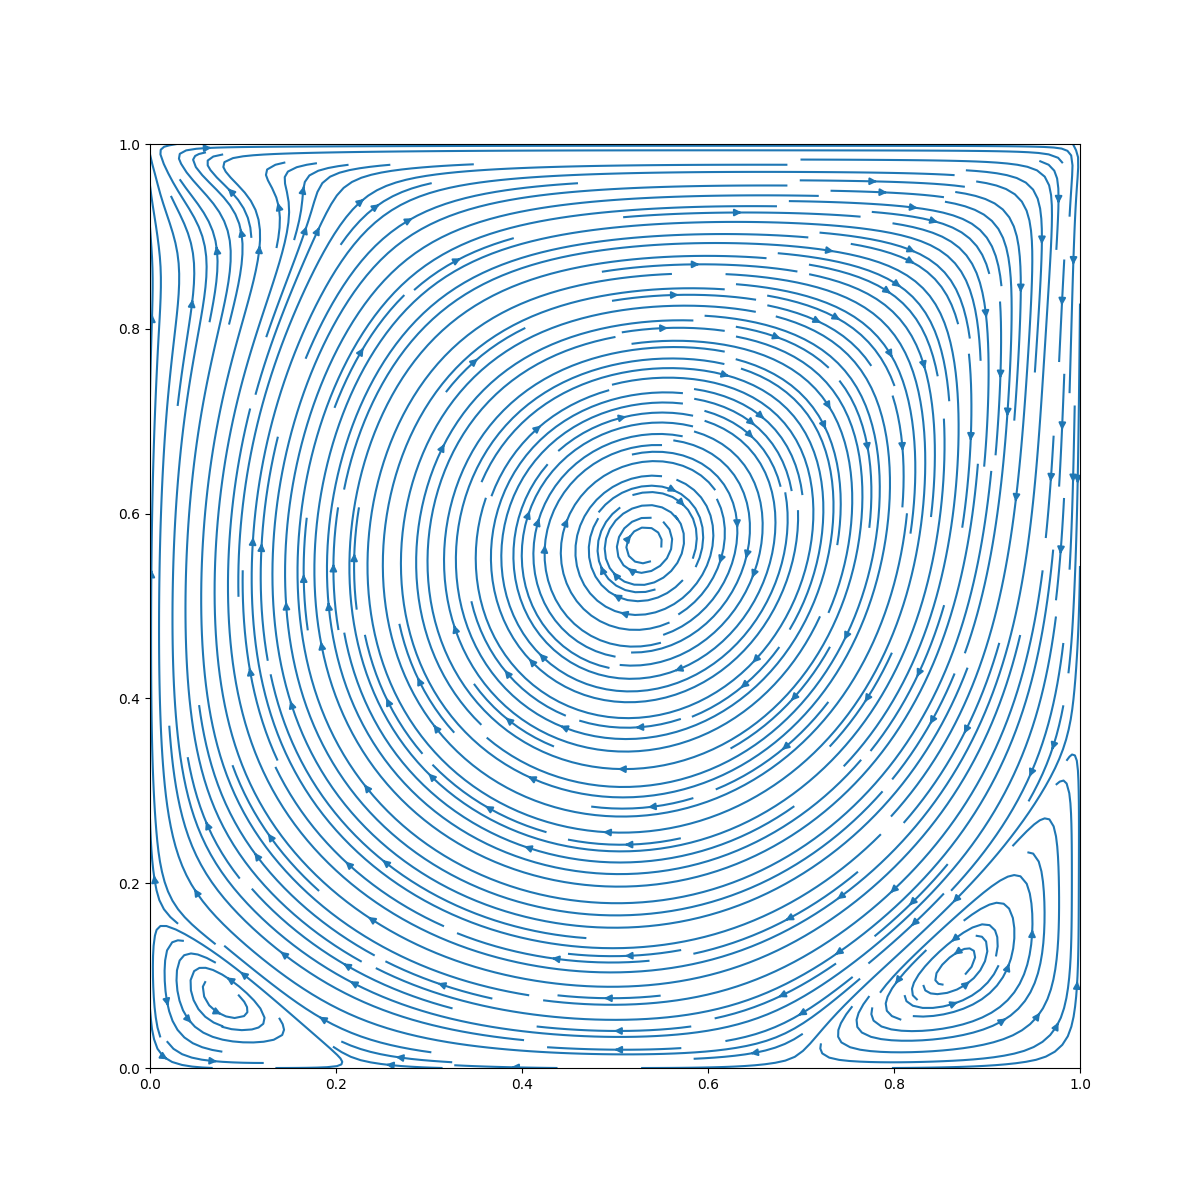
\includegraphics[width=\linewidth]{figures/Re=1000_result/Re1000_streamline_128.png}
        \caption{N=128}
    \end{subfigure}
    \caption{Stream line visualizations for Re=1000 at different grid resolutions}
\end{figure}

For Re=1000, could see the main vortex 
is still at the center, while the two 
small voetex at the left bottom and 
right bottom is also present, 
but compare to the result at Re=100, 
could also find there is a small curvature 
at the top left, while it is showing 
more obvious at the finer grid.



\subsection{Result comparison to the reference}

\subsubsection{Velocity at geometry center}

Measure our result's accuracy need us to compare the result with the reference (Ghia et al. 1982)\cite{GHIA1982387}. By compare the result at geometry center, we could check the accuracy of our result. 


\begin{figure}[H]
    \centering
    \begin{tikzpicture}
        \node[anchor=south west,inner sep=0] (image) at (0,0) {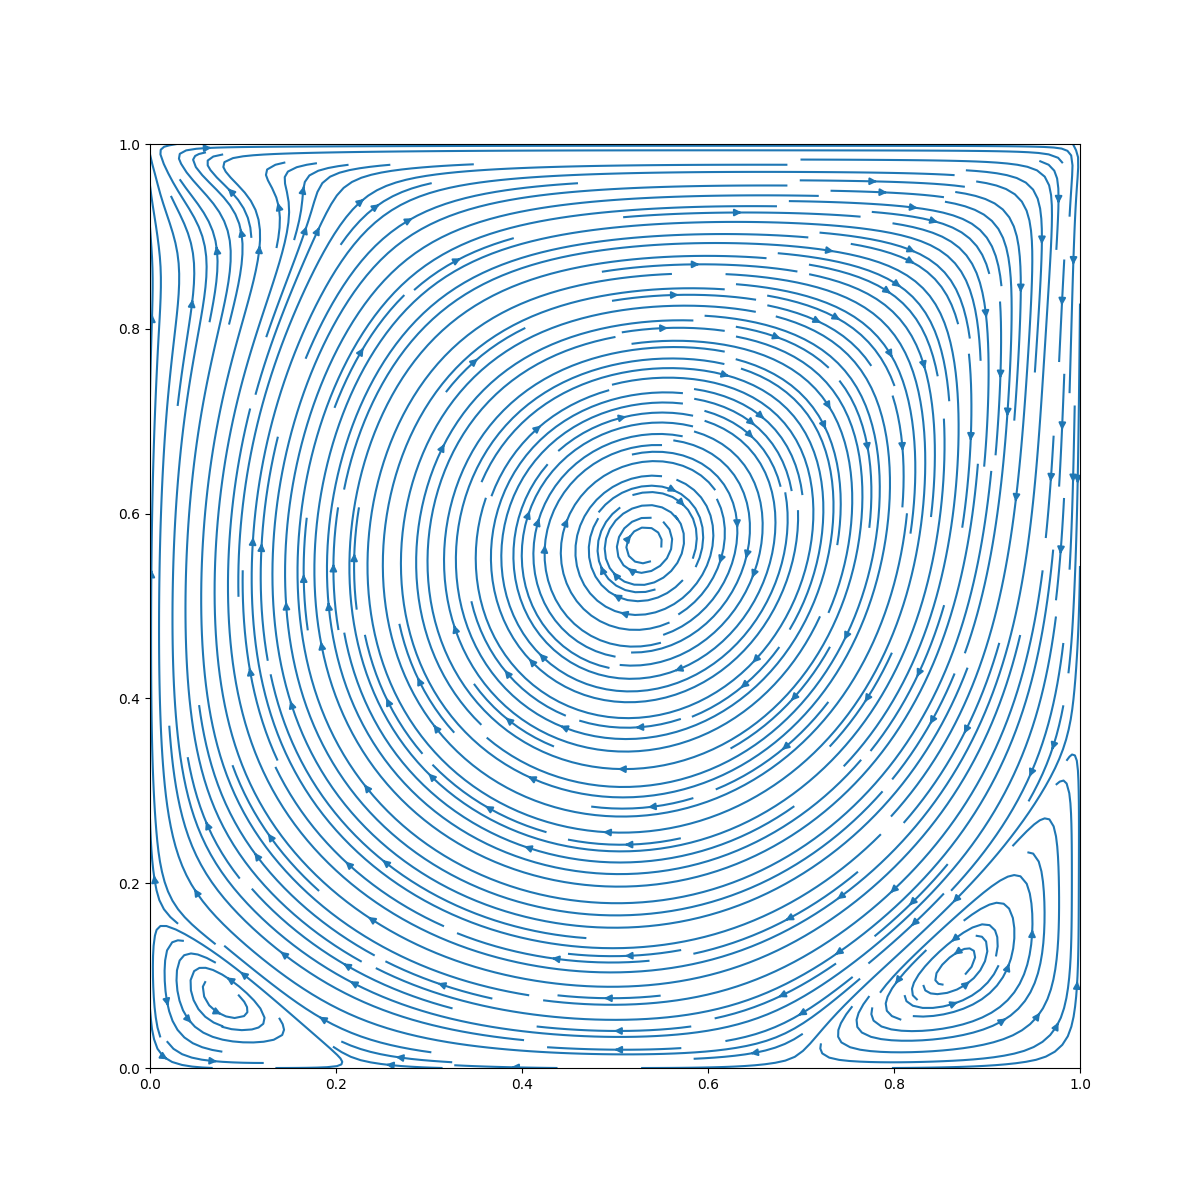
\includegraphics[width=0.6\textwidth]{figures/Re=1000_result/Re1000_streamline_128.png}};
        \begin{scope}[x={(image.south east)},y={(image.north west)}]
            % horizontal line
            \draw[black, thick] (0.1,0.5) -- (0.9,0.5);
            \node[anchor=south, align= center, text width=2cm] at (1,0.5) {v at vertical center};
            % vertical line
            \draw[black, thick] (0.5,0.1) -- (0.5,0.9);
            \node[anchor=south] at (0.5,0.05) {u at horizontal center};
        \end{scope}
    \end{tikzpicture}
    \caption{velocity at geometry center}
\end{figure}

At Re=1000, we use the the horizontal velocity u at horizontal center (at same vertical line, middle at horizontal), and vertical velocity v at vertical center (at same horizontal line, middle at horizontal). The general result is showing below:

\begin{figure}[H]
    \centering
    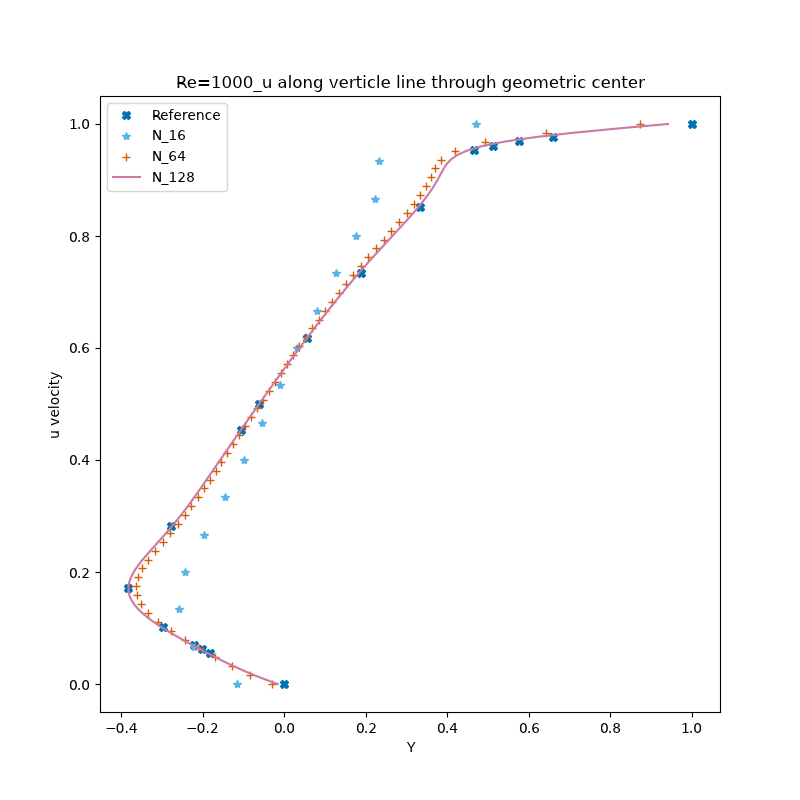
\includegraphics[width=0.5\linewidth]{figures/Re=1000_u along verticle line through geometric center.png}
    \hspace{-8mm} % Reduce horizontal space
    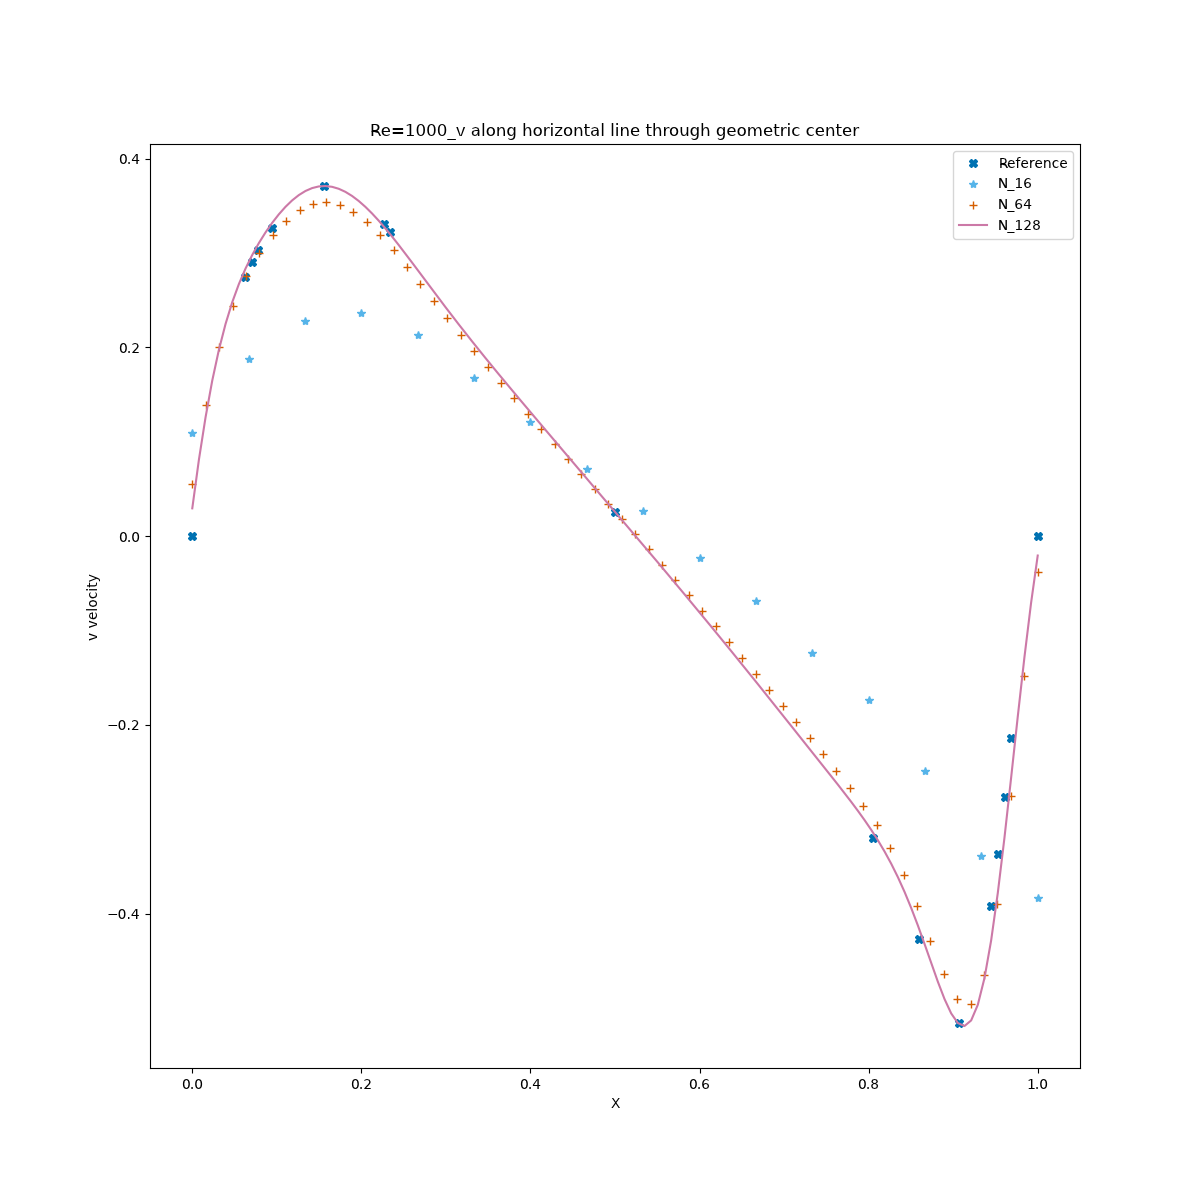
\includegraphics[width=0.5\linewidth]{figures/Re=1000_v along horizontal line through geometric center.png }
    \caption{u along vertical line at middle of x (left), v along horizontal line at middle of y (right). There is also enlarged figures showing down below.}
\end{figure}




% The graphs showing is the general view of the result comparsion, where deep blue is for the result obtained by Ghia (1982). Could say in general, the results match pretty close.


\begin{figure}[H]
    \centering
    \begin{tikzpicture}[spy using outlines={circle, magnification=2, size=6cm, connect spies}]
        \node {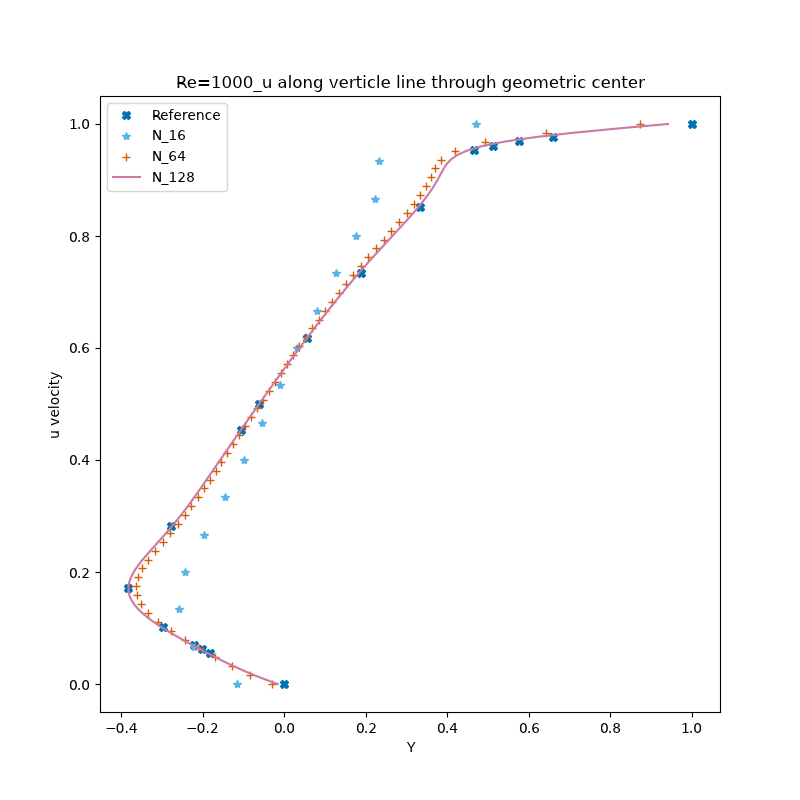
\includegraphics[width=0.6\textwidth]{figures/Re=1000_u along verticle line through geometric center.png}};
        \spy on (-2cm, -2cm) in node [left] at (6cm, -2cm);
    \end{tikzpicture}
    \caption{u along vertical line at middle of x (large)}
\end{figure}

This figures shows velocity u at the horizontal middle of the domain. Could say, in general the result is matching. Also compare different grid size, could find the coarse grid, N=16, biased largest from reference result. Conversely, the finest grid, N=128, match pretty good.


\begin{figure}[H]
    \centering
    \begin{tikzpicture}[spy using outlines={circle, magnification=2, size=4cm, connect spies}]
        \node {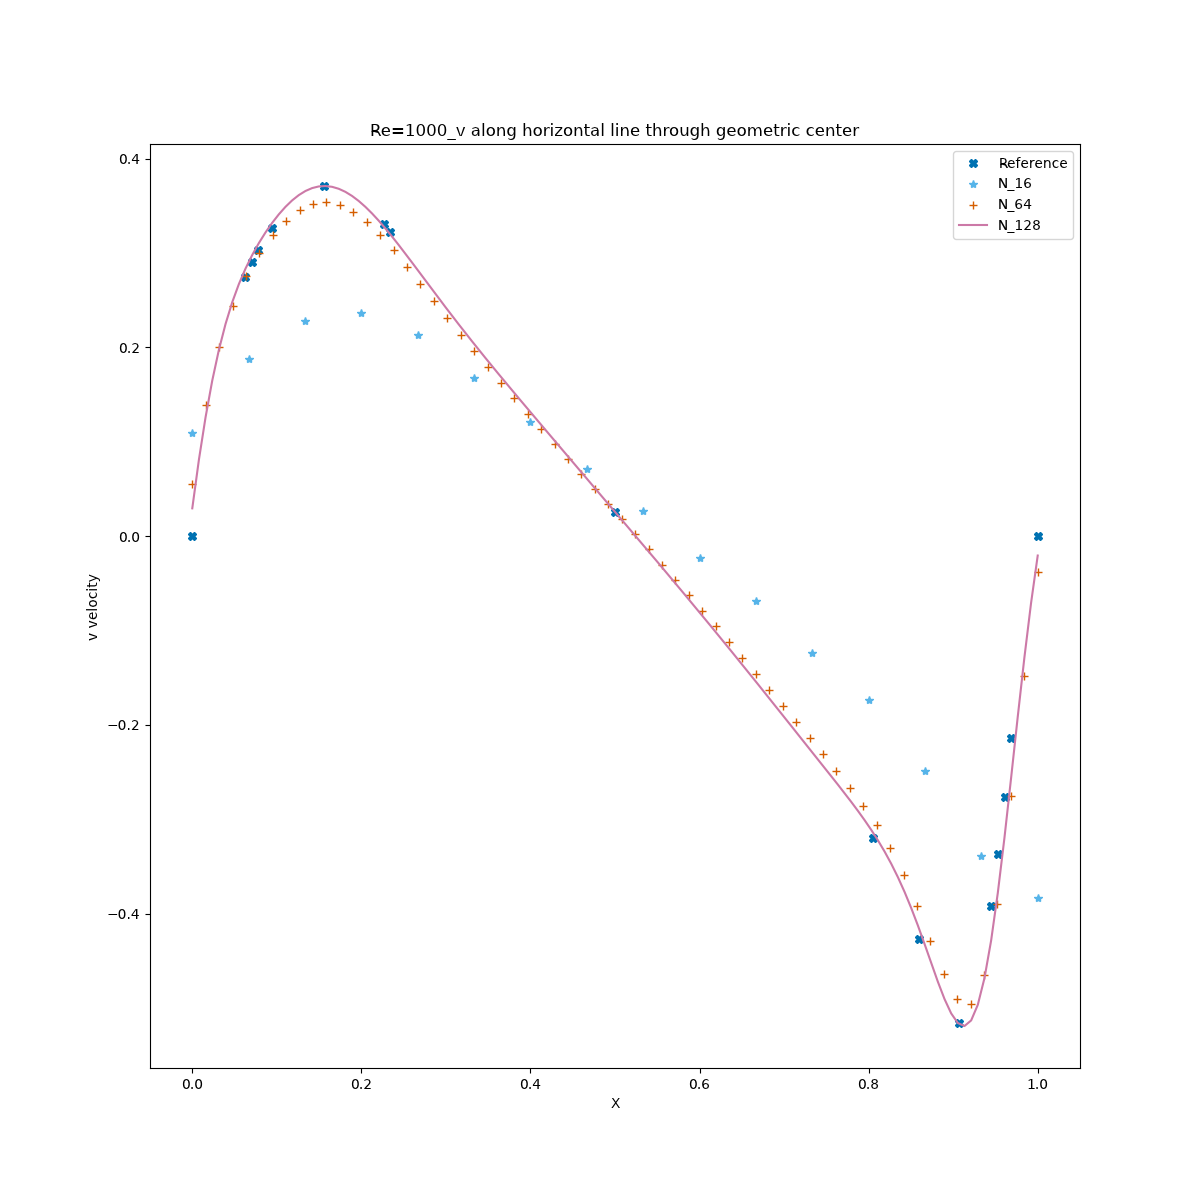
\includegraphics[width=0.6\textwidth]{figures/Re=1000_v along horizontal line through geometric center.png}};
        \spy on (-2.2cm, 2.6cm) in node [left] at (0cm, -1.5cm);
        \spy on (3cm, -2.7cm) in node [right] at (3cm, 2cm);
    \end{tikzpicture}
    \caption{v along horizontal line at middle of y (large)}
\end{figure}

We also have very similar observation on the vertical velocity v on the vertical geometry center. Could find as the grid become finer, the result match better.


\subsubsection{Streamline comparison}
\begin{figure}[H]
    \centering
    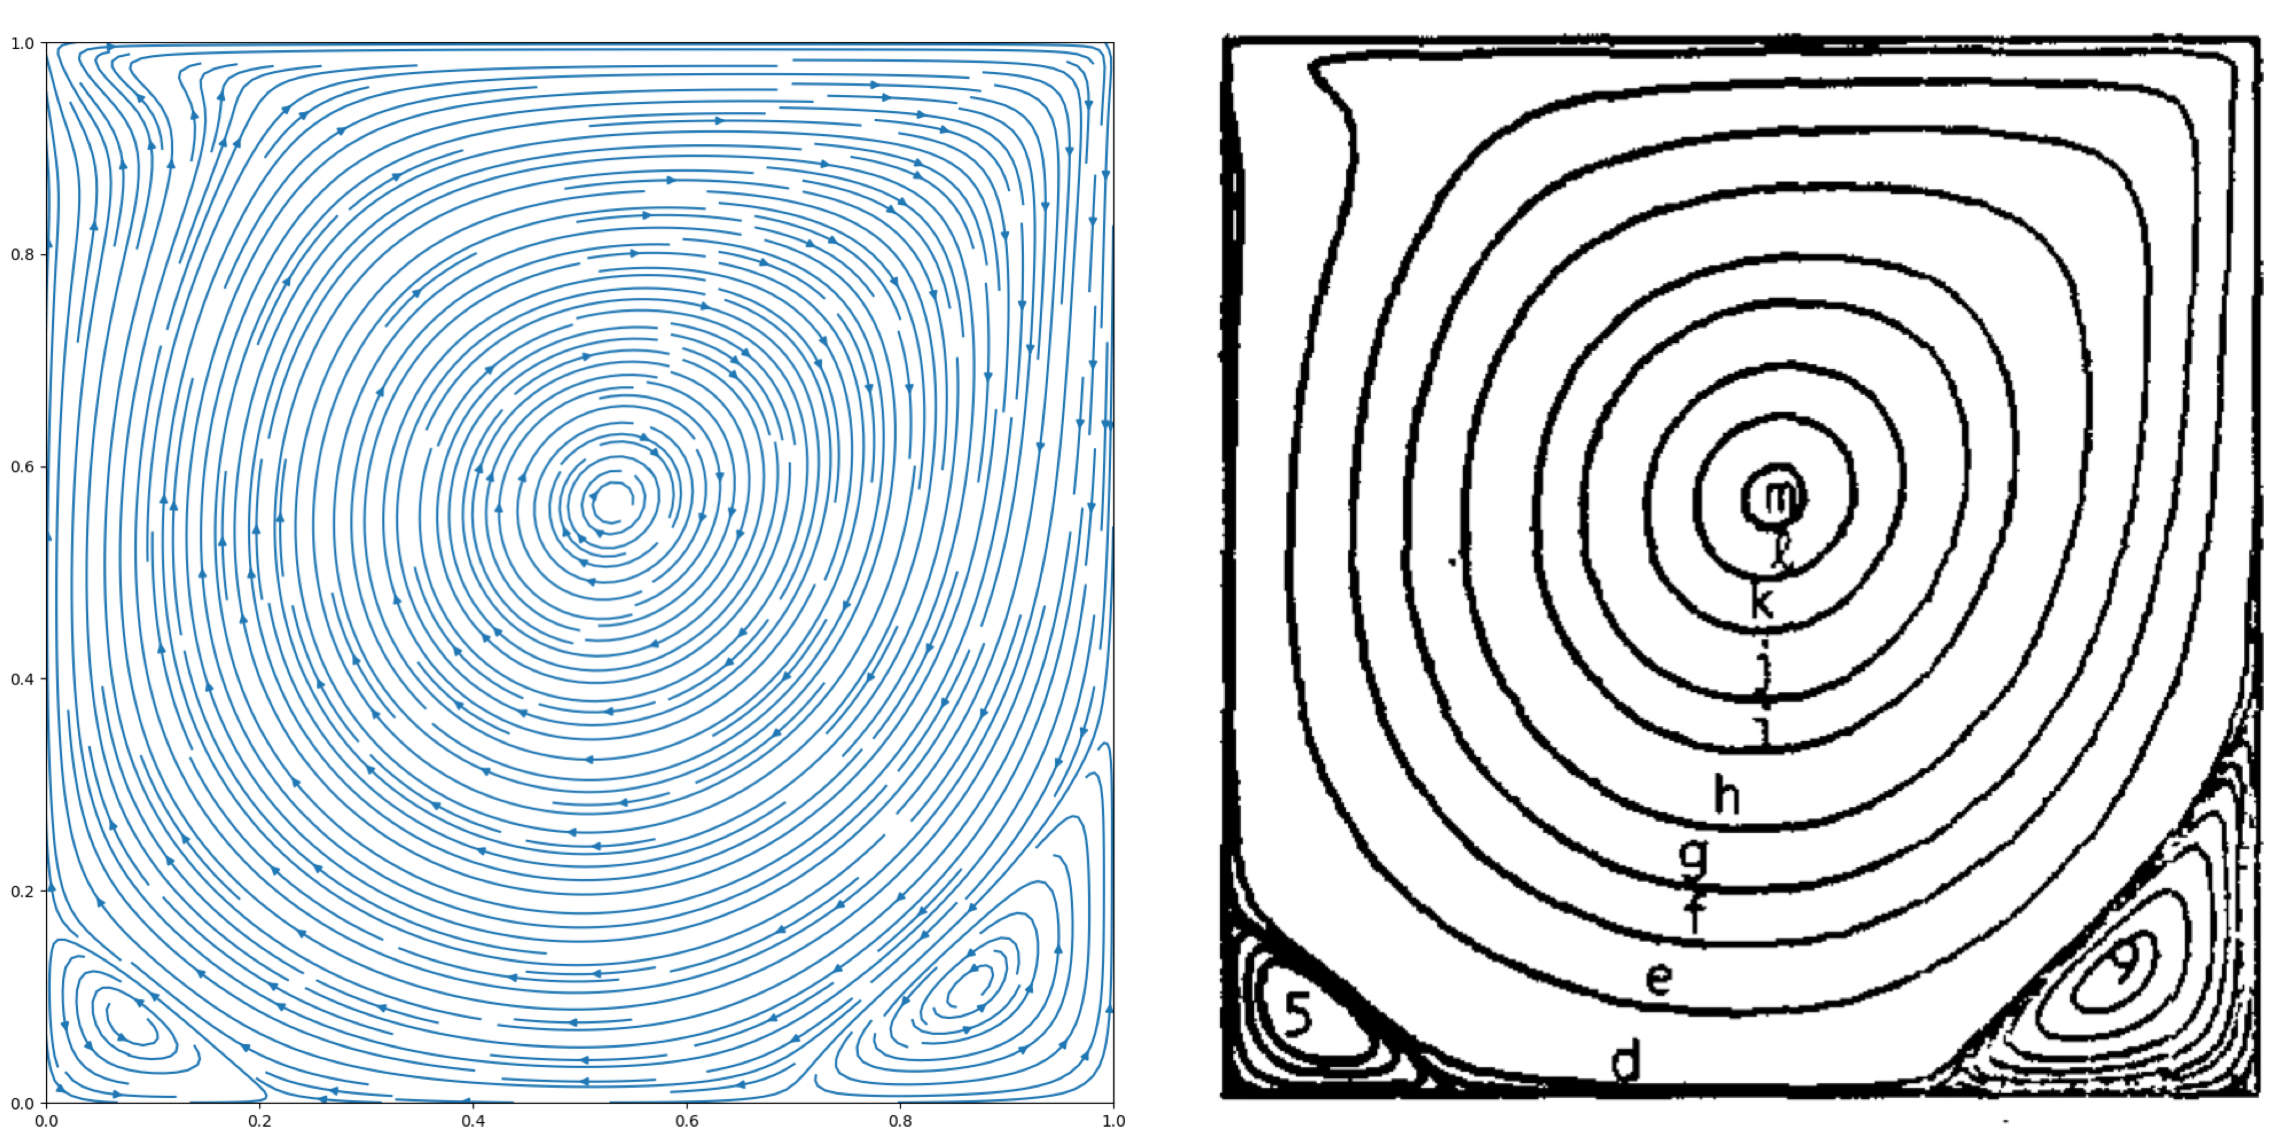
\includegraphics[width=0.9\linewidth]{Homeworks/HW4-Lid_Driven_Cavity/Latex/figures/Re=1000_result/Re=1000_Compare.jpg}
    \caption{left: Result Streamline, right: Ghia(1982)\cite{GHIA1982387}'s result}
\end{figure}

Could say the results are matching, where the vortex location and the shape are similar.
















% \begin{figure}[H]
%     \centering
%     \begin{tikzpicture}[spy using outlines={circle, magnification=2, size=6cm, connect spies}]
%         \node {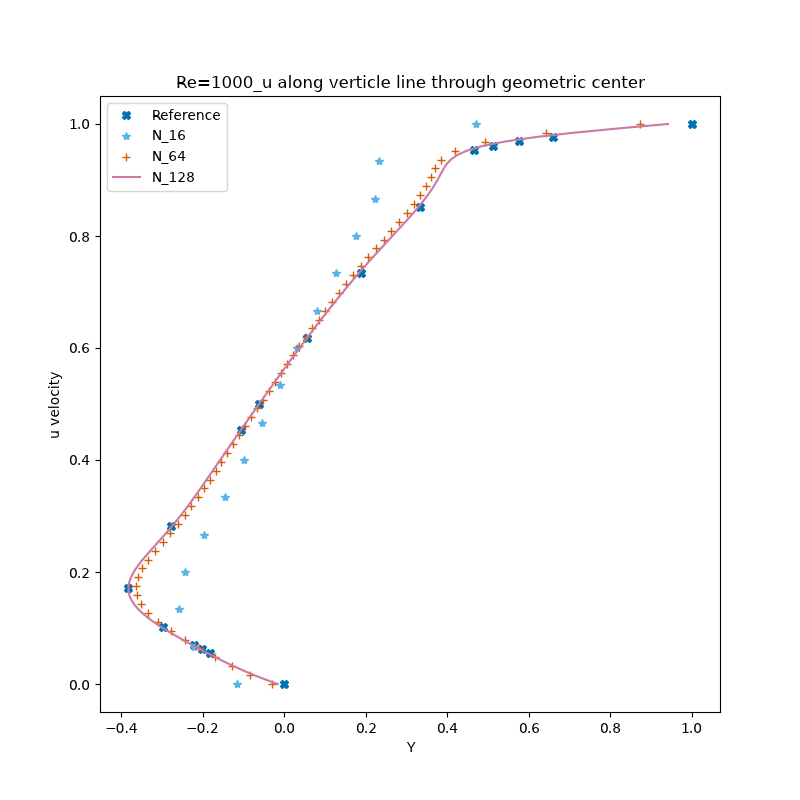
\includegraphics[width=0.9\textwidth]{figures/Re=1000_u along verticle line through geometric center.png}};
%         \spy on (-3.8cm, -3.2cm) in node [left] at (6cm, -2cm);
%     \end{tikzpicture}
%     \caption{u along vertical line at middle of x (large)}
% \end{figure}


% \begin{figure}[H]
%     \centering
%     \begin{tikzpicture}[spy using outlines={circle, magnification=2, size=4cm, connect spies}]
%         \node {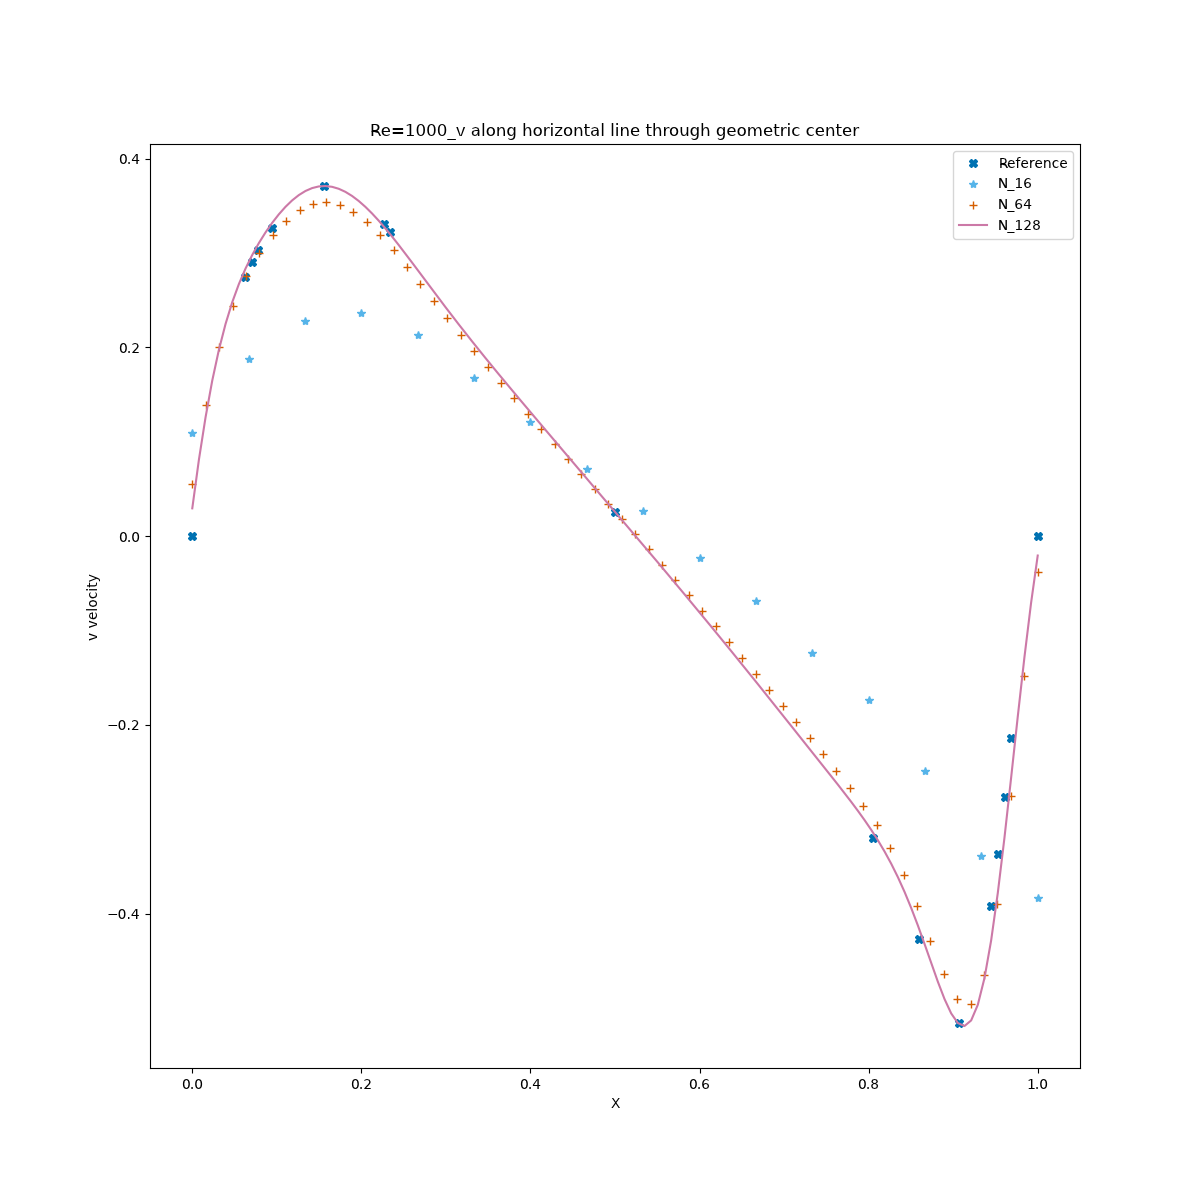
\includegraphics[width=0.9\textwidth]{figures/Re=1000_v along horizontal line through geometric center.png}};
%         \spy on (-3.2cm, 4.4cm) in node [left] at (0cm, -2cm);
%         \spy on (4.2cm, -4.4cm) in node [right] at (1cm, 2cm);
%     \end{tikzpicture}
%     \caption{v along horizontal line at middle of y (large)}
% \end{figure}





















% \begin{figure}[h]
%     \centering
%     \begin{tikzpicture}[spy using outlines={circle, magnification=2, size=3cm, connect spies}]
%         \node {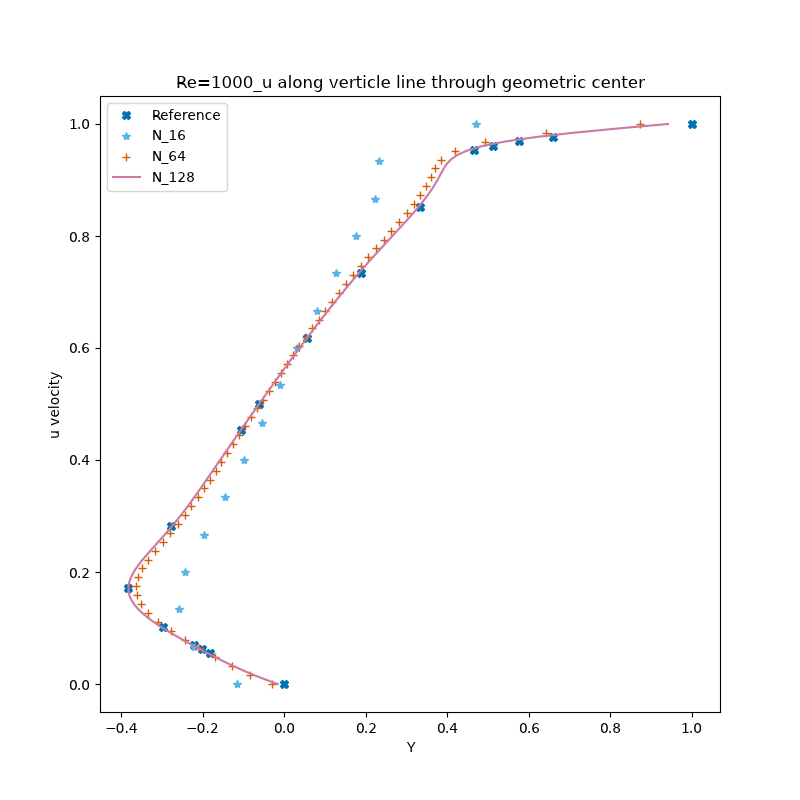
\includegraphics[width=0.48\textwidth]{figures/Re=1000_u along verticle line through geometric center.png}};
%         \spy on (-2.1cm, -1.8cm) in node [left] at (3cm, -1cm);
%     \end{tikzpicture}
%     \caption{Larger}
% \end{figure}

% \begin{figure}[h]
%     \centering
%     \begin{tikzpicture}[spy using outlines={circle, magnification=2, size=3cm, connect spies}]
%         \node {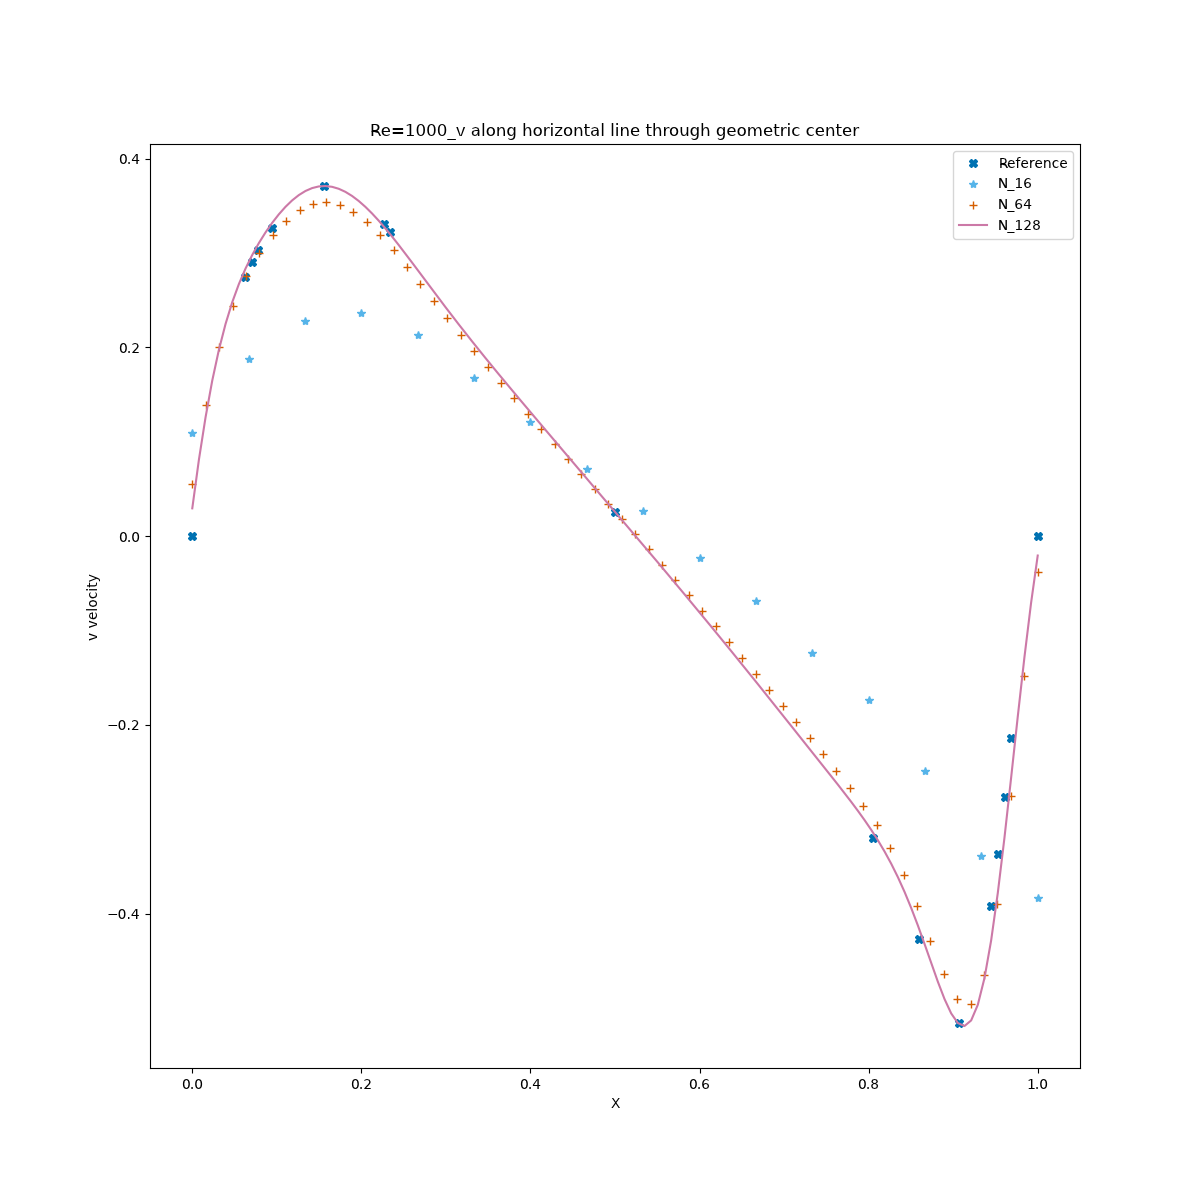
\includegraphics[width=0.48\textwidth]{figures/Re=1000_v along horizontal line through geometric center.png}};
%         \spy on (-1.8cm, 2cm) in node [left] at (0.5cm, -1cm);
%     \end{tikzpicture}
%     \caption{Larger}
% \end{figure}




% \begin{figure}[h!]
%     \centering
%     \begin{subfigure}[b]{0.45\textwidth}
%         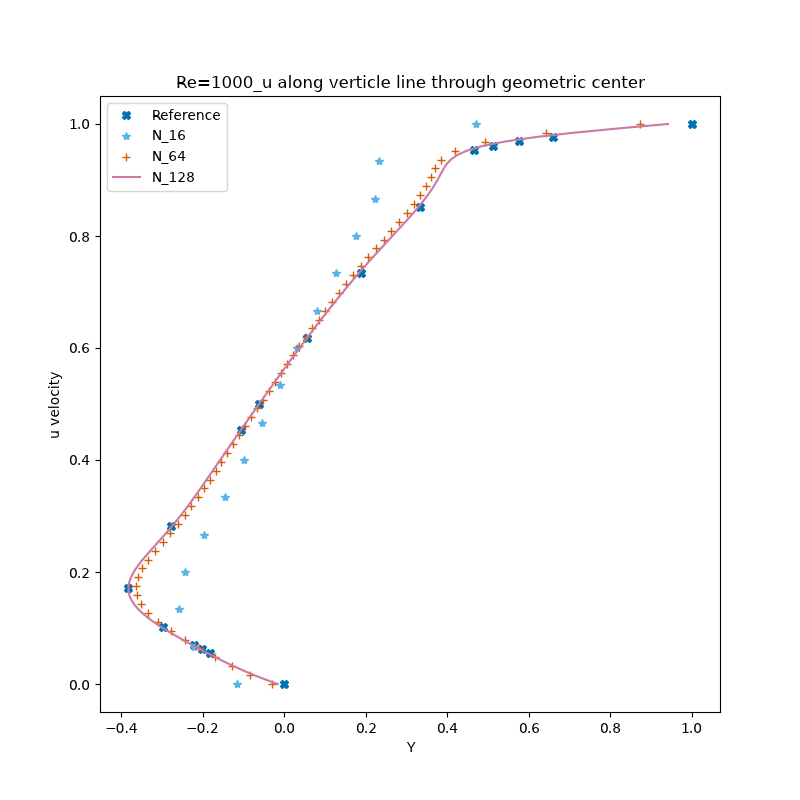
\includegraphics[width=\textwidth]{figures/Re=1000_u along verticle line through geometric center.png}
%         \caption{old}
%     \end{subfigure}
%     \hfill
%     \begin{subfigure}[b]{0.45\textwidth}
%         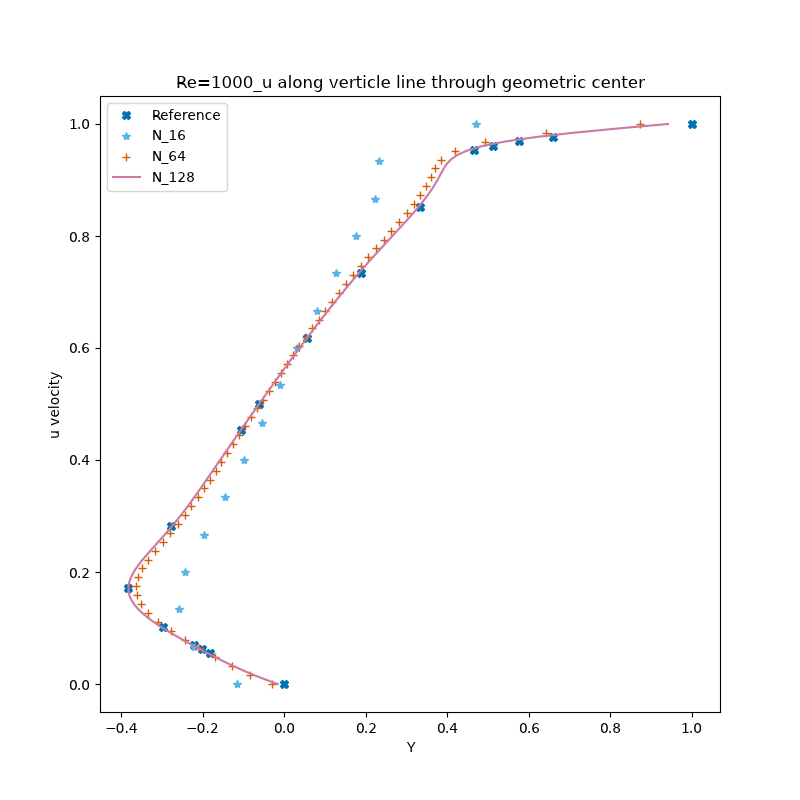
\includegraphics[width=\textwidth]{figures/Re=1000_u along verticle line through geometric center.png}
%             \caption{new}
% \end{subfigure}
% \caption{old, new}
% \end{figure}







\bibliographystyle{plain}
\bibliography{ref}
% \cite{GHIA1982387}
% \cite{BOTELLA1998421}





%%%%%%%%%%%%%%%%%%%%%%%%%%%%%%%%%%%%%%%%%%%%%%%%%%%%%%%%%%%%%%%
%%%%%%%%%%%%%%%%%%%%%%%%%%%%%%%%%%%%%%%%%%%%%%%%%%%%%%%%%%%%%%%
%%%%%%%%%%%%%%%%%%%%%%%%%%%%%%%%%%%%%%%%%%%%%%%%%%%%%%%%%%%%%%%
\newpage
\section*{Appendix}
% 在目录中添加Appendix
\addcontentsline{toc}{section}{Appendix}
\begin{scriptsize}

Our basic Solver code is showing below:
\begin{lstlisting}[language=python,caption={Lid Driven Cavity Solver}]
# This solver is a new attempt using same size of u, U... , 
# keep updating ghost point and dont need to change formula

import numpy as np
import math
import matplotlib.pyplot as plt


def TDMA(a, b, c, d):  # TDMA Solver, input abcd in same length
    # a[0], c[-1] not been used
    do = d.copy()
    ao = a.copy()
    bo = b.copy()
    co = c.copy()
    N = len(d)
    xo = np.zeros(N)
    for rowi in range(1,N):
        k = ao[rowi]/bo[rowi-1]
        bo[rowi] -= co[rowi-1]*k
        do[rowi] -= do[rowi-1]*k
    xo[N-1] = do[N-1]/bo[N-1]
    for rowi in range(N-2,-1,-1):
        xo[rowi] = (do[rowi]-co[rowi]*xo[rowi+1])/bo[rowi]
    return xo


def general_grid_generator(len_x, Nx, Ny):
    # Creating same size of u, v, U, V
    # where col 0, row 0, row -1, of U not used
    # where row 0, col 0, col -1, of V not used
    initial_Value = 0.01

    dx = len_x/Nx
    grid = np.full((Nx+2, Ny+2), initial_Value)
    u,v,U,V = data_copy(grid, grid, grid, grid)
    p = np.copy(grid)
    return u, v, U, V, p, dx

def data_copy(u, v, U, V):
    return np.copy(u), np.copy(v), np.copy(U), np.copy(V)

def Ghost_BC(u,v): # updating ghost point based on BC condition
    # (u_indomain + u_ghost)/2 = Boundary_value
    # u_ghost = 2 * Boundary_value - u_indomain
    u[-1,:] = 2*1 - u[-2,:] # upper BC
    v[-1,:] =  - v[-2,:]

    u[0, :] =  - u[1,:] # bottom BC
    v[0, :] =  - v[1,:]

    u[1:-1, 0] =  - u[1:-1,1] # left BC
    v[1:-1, 0] =  - v[1:-1,1]

    u[1:-1, -1] =  - u[1:-1,-2] # right BC
    v[1:-1, -1] =  - v[1:-1,-2]
    return u, v


def Ghost_BC_p(p): # updating ghost point for p based on BC condition
    p[-1,:] =   p[-2,:] # upper BC
    p[-1,:] =   p[-2,:]

    p[0, :] =   p[1,:] # bottom BC
    p[0, :] =   p[1,:]

    p[1:-1, 0] =   p[1:-1,1] # left BC
    p[1:-1, 0] =   p[1:-1,1]

    p[1:-1, -1] =   p[1:-1,-2] # right BC
    p[1:-1, -1] =   p[1:-1,-2]
    return p



def UV_BC(U, V):
    U[1:-1,1] = 0
    U[1:-1,-1] = 0
    V[1,1:-1] = 0
    V[-1,1:-1] = 0
    return U,V



def coeff_assemble(rows_cols, a_e, b_e, c_e, e_e, f_e):
    rows, cols = rows_cols[0], rows_cols[1]
    # input elements of abcdef, get line matrix of abcdef
    a = np.full((rows, cols), a_e ) # abc in same length of Ncols of u
    b = np.full((rows, cols), b_e )
    c = np.full((rows, cols), c_e )

    e = np.full((rows, cols), e_e ) # ef in same length of Nrows of u
    f = np.full((rows, cols), f_e )
    a[:,0]= a[:,-1] = c[:,0] = c[:,-1] = 0
    b[:,0] = b[:,-1] = 1
    e[:,-1] =e[:,0] = f[:,-1]= f[:,0]=0
    return a,b,c, e,f



def RHS_uv(f, f_old, U, V, U_old, V_old, c0, r): 
    # Update Right Hand Side
    f_P = f[1:-1,1:-1]
    f_W = f[1:-1,:-2]
    f_E = f[1:-1,2:]
    f_S = f[:-2,1:-1]
    f_N = f[2:,1:-1]

    f_P_old = f_old[1:-1,1:-1]
    f_W_old = f_old[1:-1,:-2]
    f_E_old = f_old[1:-1,2:]
    f_S_old = f_old[:-2,1:-1]
    f_N_old = f_old[2:,1:-1]

    convection_new = c0*( U[1:-1,2:] * (f_E + f_P)/2 -
                          U[1:-1,1:-1] * (f_W + f_P)/2 +
                          V[2:,1:-1]  * (f_N + f_P)/2 -
                          V[1:-1,1:-1] * (f_S + f_P)/2 )
    
    convection_old = c0*( U_old[1:-1,2:] * (f_E_old + f_P_old)/2 -
                          U_old[1:-1,1:-1] * (f_W_old + f_P_old)/2 +
                          V_old[2:,1:-1]  * (f_N_old + f_P_old)/2 -
                          V_old[1:-1,1:-1] * (f_S_old + f_P_old)/2 )
    
    diffusion = f_P + r*(f_E + f_W + f_N + f_S -4*f_P)
    return -3/2*convection_new + 1/2*convection_old + diffusion

def Not_Use_UV_BC(U,V):
    U[0,:] = U[-1,:] = U[:,0] = V[:,0] = V[:,-1] = V[0,:] = -10000
    return U,V

def Residual(u, a, b, c, d, e, f):
    Res = np.zeros_like(u)
    Res[1:-1,1:-1] = (a[1:-1,1:-1] * u[1:-1,:-2] +
                      b[1:-1,1:-1] * u[1:-1,1:-1] +
                      c[1:-1,1:-1] * u[1:-1,2:] +
                      e[1:-1,1:-1] * u[:-2,1:-1] +
                      f[1:-1,1:-1] * u[2:,1:-1] -
                      d[:,:])
    # print(Res)
    return Res


def Point_GS(a,b,c,d,e,f,u):
    u_k = np.copy(u)
    u_k_new = np.copy(u)
    n_rows = np.size(u,0)
    w = 1.9
    D = np.zeros_like(a[1,:])
    Res = 100
    k = 0
    while Res>1e-6:
        u_k = np.copy(u_k_new) 
        u_k_new[1:-1,1:-1] = (-a[1:-1,1:-1] * u_k_new[1:-1,:-2] +
                              -c[1:-1,1:-1] * u_k[1:-1,2:] +
                              -e[1:-1,1:-1] * u_k_new[:-2,1:-1] +
                              -f[1:-1,1:-1] * u_k[2:,1:-1] +
                              d[:,:])/b[1:-1,1:-1]
        u_k_new[1:-1] = u[1:-1]*(1-w) + u_k_new[1:-1]*w # SOR term
        
        Res = np.linalg.norm(Residual(u_k_new, a, b, c, d, e, f))
        # print("Res=")
        # print(Res) 
        if Res > 1e+200: 
            print("NOT CONVERGE NOT CONVERGE NOT CONVERGE NOT CONVERGE") 
            print(Res)
            quit()
        u = np.copy(u_k)
        k+=1
    # print("finish iteration")
        
    return u_k_new, k



def LineSOR(a,b,c,d,e,f, u): 
    # input abcdef, and u, get D
    # then use TDMA get new u
    # abc is in same size of N_rows of u, ef in same size of N_cols of u
    # ! Input d is LIKE inner field of u, need to cut each line to use !
    u_k = np.copy(u)
    u_k_new = np.copy(u)
    n_rows = np.size(u,0)
    w = 1.9
    D = np.zeros_like(a[1,:])
    Res = 100
    while Res>1e-6:
        u_k = np.copy(u_k_new) 
        for j in range(1,n_rows-1): # the number is based on d, which is (N-1)x(N-1)
            # D = np.zeros_like(a[1,:])
            D[1:-1] = d[j-1,:] - e[j,1:-1]*u_k_new[j-1,1:-1] - f[j,1:-1]*u_k[j+1,1:-1]
            D[0], D[-1] = u[j,0], u[j,-1] # ghost point = ghost point
            u_k_new[j,:] = TDMA(a[j,:],b[j,:],c[j,:],D) # TDMA solve uk each line
            # u_k_new[j,:] = u[j,:]*(1-w) + TDMA(a,b,c,D)*w # SOR term
        
        Res = np.linalg.norm(Residual(u_k_new, a, b, c, d, e, f))
        # print("Res=")
        # print(Res) 
        if Res > 1e+20: 
            print("NOT CONVERGE NOT CONVERGE NOT CONVERGE NOT CONVERGE") 
            quit()
        u = np.copy(u_k)
    # print("finish iteration")
    return u_k_new




def Solver(u, v, U, V, p, t, dt, dx, Re):
    r = dt/(2*Re*dx**2)
    c0 = dt/(dx)
    
    rows_cols = np.shape(u)
    a_uv,b_uv,c_uv,e_uv,f_uv  = coeff_assemble(rows_cols, -r, 1+4*r, -r, -r, -r)
    a_p,b_p,c_p,e_p,f_p  = coeff_assemble(rows_cols, 1, -4, 1, 1, 1)

    U, V = UV_BC(U, V)
    u, v = Ghost_BC(u,v)

    U, V = Not_Use_UV_BC(U, V) 

    u_star, v_star, U_star, V_star = data_copy(u, v, U, V) 
    u_new, v_new, U_new, V_new = data_copy(u, v, U, V) 
    u_old, v_old, U_old, V_old = data_copy(u, v, U, V)


    # n_max = int(t/dt)
    Difference = 100

    n=0
    while Difference>1e-6:
        U, V = UV_BC(U, V) # Setup BC

        # Step 1: get u_star, v_star, U_star, V_star
        u, v = Ghost_BC(u,v)
        u_star, v_star = Ghost_BC(u_star,v_star)

        # get u_star:    
        d = RHS_uv(u, u_old, U, V, U_old, V_old, c0, r)
        u_star = LineSOR(a_uv,b_uv,c_uv, d , e_uv,f_uv, u)


        u_star, v_star = Ghost_BC(u_star,v_star)

        # get v_star:
        d = RHS_uv(v, v_old, U, V, U_old, V_old, c0, r) 
        v_star = LineSOR(a_uv,b_uv,c_uv, d , e_uv,f_uv, v)

        u_star, v_star = Ghost_BC(u_star,v_star)

        # get U_star, V_star
        U_star[1:-1,2:] =  (u_star[1:-1,1:-1] + u_star[1:-1,2:])/2
        V_star[2:,1:-1] =  (v_star[2:,1:-1] + v_star[1:-1,1:-1])/2

        U_star, V_star = UV_BC(U_star, V_star) # Setup BC


        # Step 2: get New Pressure P
        d = dx/dt * (
            U_star[1:-1, 2:] - U_star[1:-1, 1:-1] +
            V_star[2:, 1:-1] - V_star[1:-1, 1:-1]
        )
        p_new,k = Point_GS(a_p,b_p,c_p,d, e_p,f_p, p)
        p_new = Ghost_BC_p(p_new)


        # Step 3: get u_new, v_new, U_new , V_new
        # update u_new, v_new
        u_new[1:-1,1:-1] = u_star[1:-1, 1:-1] - dt/dx*(p_new[1:-1,2:] - p_new[1:-1,:-2])/2 
        v_new[1:-1,1:-1] = v_star[1:-1, 1:-1] - dt/dx*(p_new[2:,1:-1] - p_new[:-2,1:-1])/2 
        u_new, v_new = Ghost_BC(u_new,v_new)
        # update U_new , V_new
        U_new[1:-1,2:] = U_star[1:-1,2:] - dt/dx*(p_new[1:-1,2:]-p_new[1:-1,1:-1])
        V_new[2:,1:-1] = V_star[2:,1:-1] - dt/dx*(p_new[2:,1:-1]-p_new[1:-1,1:-1])
        U_new, V_new = UV_BC(U_new, V_new) # Setup BC

        # print('new done')

        u_old, v_old, U_old, V_old = data_copy(u, v, U, V)
        u, v, U, V = data_copy(u_new, v_new, U_new, V_new)
        N = rows_cols[1]-2
        Difference = np.sum(np.abs(u - u_old)+np.abs(v - v_old)+np.abs(p_new - p))/N**2

        p = np.copy(p_new)

        # print(Big_Res)
        n +=1
        print("time=%.3f, Difference=%.9f, p iteration times=%d"%((n+1)*dt,Difference,k))
    return u, v, p



def draw_streamline(u, v, len_x, len_y ,label):
    rows, cols = np.shape(u)  
    X = np.linspace(0, len_x, cols)
    Y = np.linspace(0, len_y, rows)
    plt.figure(figsize=(12, 12))
    plt.streamplot(X, Y, u, v, density =3)
    plt.axis([0,1,0,1])
    plt.title(f'streamline_{label}')
    plt.savefig(f'streamline_{label}.png')
    # plt.show()


def draw_velocity_contour(u, v, len_x, len_y,label):
    levels=100 
    rows, cols = np.shape(u)
    X, Y = np.linspace(0, len_x, cols), np.linspace(0, len_y, rows)
    velocity_magnitude = np.sqrt(u**2 + v**2)
    plt.figure(figsize=(12, 12))
    plt.contourf(X, Y, velocity_magnitude, levels=levels, cmap='jet')
    plt.colorbar(label='Velocity magnitude')
    plt.xlabel('X')
    plt.ylabel('Y')
    plt.title(f'velocity_contour_{label}')
    plt.savefig(f'velocity_contour_{label}.png')
    # plt.show()


def draw_u_contour(u, v, len_x, len_y ,label):
    levels=100
    rows, cols = np.shape(u)
    X, Y = np.linspace(0, len_x, cols), np.linspace(0, len_y, rows)
    plt.figure(figsize=(12, 12))
    plt.contourf(X, Y, u, levels=levels, cmap='jet')
    plt.colorbar(label='u magnitude')
    plt.xlabel('X')
    plt.ylabel('Y')
    plt.title(f'u_contour_{label}')
    plt.savefig(f'u_contour_{label}.png')
    # plt.show()



def save(u,v,p,label):
    with open(f'output_N={label}.txt', 'w') as f:
        f.write(f'For grid size N= {label}:\n')
        f.write('Array u:\n')  
        f.write(','.join(map(str, u)) + '\n\n')  
        f.write('Array v:\n')  
        f.write(','.join(map(str, v)) + '\n\n')  
        f.write('Array p:\n')  
        f.write(','.join(map(str, p)) + '\n')  



def main():
    N = 32
    t = 20



    dt = 0.02

    len_x = 1
    len_y = 1
    Nx = Ny = N
    Re = 100

    u, v, U, V, p, dx = general_grid_generator(len_x, Nx, Ny)

    u,v, p =Solver(u, v, U, V, p, t, dt, dx, Re)

    print(u)
    print(v)
    print(p)

    save(u,v,p,N)
    

    
    draw_streamline(u[1:-1,1:-1],v[1:-1,1:-1], len_x, len_y , N)
    draw_velocity_contour(u[1:-1,1:-1],v[1:-1,1:-1], len_x, len_y , N)
    draw_u_contour(u[1:-1,1:-1],v[1:-1,1:-1], len_x, len_y , N)




if __name__ == '__main__':
    main()





\end{lstlisting}





\begin{lstlisting}[language=python,caption={Post Operator:}]
import numpy as np
import re
import matplotlib.pyplot as plt

def load_2d_arrays_with_numpy(label):
    filename = f'output_N={label}.txt'
    try:
        with open(filename, 'r') as file:
            content = file.read()
    except FileNotFoundError:
        print("文件未找到,请检查文件路径是否正确")
        return None, None, None

    # 辅助函数来提取并构建二维数组
    def extract_2d_array(array_content):
        array_data = []
        # 匹配方括号内的所有内容,包括可能的多行
        matches = re.findall(r'\[(.*?)]', array_content.replace('\n', ''), re.DOTALL)
        for match in matches:
            # 替换掉可能存在的换行符,然后解析数值
            formatted_match = ' '.join(match.split())
            numbers = np.fromstring(formatted_match, sep=' ')
            array_data.append(numbers)
        return np.array(array_data)

    # 改进正则表达式以匹配整个数组块
    u_data = re.search(r'Array u:\s*((?:\[\s*.*?\s*\][,\s]*)+)', content, re.DOTALL)
    v_data = re.search(r'Array v:\s*((?:\[\s*.*?\s*\][,\s]*)+)', content, re.DOTALL)
    p_data = re.search(r'Array p:\s*((?:\[\s*.*?\s*\][,\s]*)+)', content, re.DOTALL)

    if not (u_data and v_data and p_data):
        print("未能正确提取u, v, 或 p的数据。请检查数组标记和文件格式。")
        return np.array([]), np.array([]), np.array([])

    u = extract_2d_array(u_data.group(1))
    v = extract_2d_array(v_data.group(1))
    p = extract_2d_array(p_data.group(1))

    return u, v, p

def smalluvp(u,v,p):
    return u[1:-1,1:-1],v[1:-1,1:-1],p[1:-1,1:-1] 

def Center(u,v,p, label):
    u,v,p = smalluvp(u,v,p)
    
    center = int(label/2)
    u_x_center = (u[:,center] + u[:,center-1])/2
    v_x_center = (v[:,center] + v[:,center-1])/2
    p_x_center = (p[:,center] + p[:,center-1])/2

    u_y_center = (u[center,:] + u[center-1,:])/2
    v_y_center = (v[center,:] + v[center-1,:])/2
    p_y_center = (p[center,:] + p[center-1,:])/2

    return u_x_center, v_x_center, p_x_center\
    ,u_y_center, v_y_center, p_y_center


# def drawing(u_x_c, u_y_c):
    
    
def get_ue_x_c():
    ye_0 = [1.00000, 0.9766, 0.9688, 0.9609, 0.9531, 0.8516, 0.7344, 0.6172, 0.5000, 0.4531, 0.2813, 0.1719, 0.1016, 0.0703, 0.0625, 0.0547, 0.0000]
    ue_x_c_0 = [1.00000, 0.84123, 0.78871, 0.73722, 0.68717, 0.23151, 0.00332, -0.13641, -0.20581, -0.21090, -0.15662, -0.10150, -0.06434, -0.04775, -0.04192, -0.03717, 0.00000]
    return ye_0[::-1], ue_x_c_0[::-1]

def get_ue_y_c():
    xe_0 = [1.0000, 0.9688, 0.9609, 0.9531, 0.9453, 0.9063, 0.8594, 0.8047, 0.5000, 0.2344, 0.2266, 0.1563, 0.0938, 0.0781, 0.0703, 0.0625, 0.0000]
    xe_y_c_0 = [0.00000, -0.05906, -0.07391, -0.08864, -0.10313, -0.16914, -0.22445, -0.24533, 0.05454, 0.17527, 0.17507, 0.16077, 0.12317, 0.10890, 0.10091, 0.09233, 0.00000]
    return xe_0[::-1], xe_y_c_0[::-1]


# def drawing(u_x_c_16, u_x_c_64, u_x_c_128):
#     ye, ue_x_c = get_ue_x_c()
#     y = np.linspace(0,N*1/N, N)
#     plt.figure(figsize=(8, 8))
#     plt.plot(ye, ue_x_c, label='Paper Result')
#     plt.plot(y, u_x_c, label='Result')
#     plt.xlabel('X')
#     plt.ylabel('u velocity')
#     plt.legend()
#     # plt.title('u Contour')
#     # plt.savefig(f'u_contour_{label}.png')
#     plt.show()


def drawing_x_c(u_x_c_16, u_x_c_64, u_x_c_128):
    ye, ue_x_c_vertical = get_ue_x_c()
    y_16 = np.linspace(0,1, 16)
    y_64 = np.linspace(0,1, 64)
    y_128 = np.linspace(0,1, 128)
    plt.figure(figsize=(8, 8))
    plt.plot( ue_x_c_vertical, ye, '-x', label='Paper Result', color= 'red')
    plt.plot( u_x_c_16,y_16, '-x', label='Result_16',color= 'blue')
    plt.plot( u_x_c_64,y_64, '-x', label='Result_64',color= 'green')
    plt.plot( u_x_c_128,y_128, '-', label='Result_128',color= 'navy')
    plt.xlabel('Y')
    plt.ylabel('u velocity')
    plt.legend()
    plt.title('u along verticle line through geometric center')
    plt.savefig('u along verticle line through geometric center')
    # plt.show()



    

def drawing_y_c(v_y_c_16, v_y_c_64, v_y_c_128):
    xe, ue_y_c_vertical = get_ue_y_c()
    plt.figure(figsize=(12,12))
    x_16 = np.linspace(0,16*1/16, 16)
    x_64 = np.linspace(0,64*1/64, 64)
    x_128 = np.linspace(0,128*1/128, 128)

    plt.plot(xe, ue_y_c_vertical, '-x', label='Paper Result',color= 'red')
    plt.plot(x_16, v_y_c_16, '-x', label='Result_16',color= 'blue')
    plt.plot(x_64, v_y_c_64, '-x', label='Result_64',color= 'green')
    plt.plot(x_128, v_y_c_128, '-', label='Result_128',color= 'navy')
    plt.xlabel('X')
    plt.ylabel('v velocity')
    plt.legend()
    plt.title('v along horizontal line through geometric center')
    plt.savefig('v along horizontal line through geometric center')
    # plt.show()


def center_get(N):
    u, v, p = load_2d_arrays_with_numpy(N)
    return Center(u,v,p, N)








def main():
    # 使用示例
    # N = 128
    # u, v, p = load_2d_arrays_with_numpy(N)
    # print(u[-2,:])
    # u_x_c, v_x_c, p_x_c, u_y_c, v_y_c, p_y_c = Center(u,v,p, N)

    u_x_c_128, v_x_c_128, p_x_c_128, u_y_c_128, v_y_c_128, p_y_c_128 = center_get(128)
    u_x_c_64, v_x_c_64, p_x_c_64, u_y_c_64, v_y_c_64, p_y_c_64 = center_get(64)
    u_x_c_16, v_x_c_16, p_x_c_16, u_y_c_16, v_y_c_16, p_y_c_16 = center_get(16)

    # drawing_x_c(u_x_c_16, u_x_c_64, u_x_c_128)
    # drawing_y_c(v_y_c_16, v_y_c_64, v_y_c_128)



if __name__ == '__main__':
    main()

    


\end{lstlisting}





















\end{scriptsize}




%%%%%%%%%%%%%%%%%%%%%%%%%%%%%%%%%%%%%%%%%%%%%%%%%%%%%%%%%%%%%%%
%%%%%%%%%%%%%%%%%%%%%%%%%%%%%%%%%%%%%%%%%%%%%%%%%%%%%%%%%%%%%%%
%%%%%%%%%%%%%%%%%%%%%%%%%%%%%%%%%%%%%%%%%%%%%%%%%%%%%%%%%%%%%%%



\end{document}